\documentclass[a4paper,12pt,twoside]{article}
\begin{filecontents*}{Animationen-und-HOP-Typ2.rkt}
; Erstellung von Animationen mit Teachpack "universe"
; (1) Zähler

(: scene (natural -> image))
(define scene
  (lambda (t)
    (text (number->string t) 100 "red")))
(big-bang 0
          (on-tick (lambda (t) (+ t 1)))
          (to-draw scene 200 100))




; Erstellung von Animationen mit Teachpack "universe"
; (2) X-Wing Fighter + Scrolling Death Star

(define death-star 
@
\includegraphics[width=\textwidth]{death-star}@)
(define x-wing @
\includegraphics{xwing}@)


; Erhalte einfachen Scrolling-Effekt durch Herausschneiden von Teilbildern
; aus dem Bild der Todessternoberfläche
; (zu crop und overlay: siehe Dokumentation des Teachpack "image2")
(: scroll-death-star (natural -> image))
(define scroll-death-star
  (lambda (t)
    (overlay x-wing
             (crop (modulo (* 8 t) 200) 0 400 440 death-star))))
(big-bang 0
          (on-tick (lambda (t) (+ t 1)))
          (to-draw scroll-death-star))


; ----------------------------------------------------------------------

; Komposition der Prozeduren f, g (Mathematik: f ∘ g, "f nach g") 
(: compose ((%b -> %c) (%a -> %b) -> (%a -> %c)))
(define compose
  (lambda (f g)
    (lambda (x)
      (f (g x)))))



; Greife auf das zweite Element der Liste xs zu
(: second ((list-of %a) -> %a))
(check-expect (second (list 1 2 3)) 2)
(check-expect (second (string->strings-list "SCF")) "C")
(define second
  (lambda (xs)
    ((compose first rest) xs)))


; Greife auf das dritte Element der Liste xs zu
(: third ((list-of %a) -> %a))
(check-expect (third  (list 1 2 3)) 3)
(check-expect (third (string->strings-list "SCF")) "F")
(define third
  (lambda (xs)
    ((compose first (compose rest rest)) xs)))


; Komponiere f n-mal mit sich selbst (fⁿ, Funktions-Exponentation)
(: repeat (natural (%a -> %a) -> (%a -> %a)))
(define repeat
  (lambda (n f)
    (cond ((= n 0) (lambda (x) x))                      ; ← Identität (id)
          ((> n 0) (compose (repeat (- n 1) f) f))))) 


; Greife auf das n-te Elemente der Liste xs zu
(: nth (natural (list %a) -> %a))
(check-expect (nth 2 (string->strings-list "SCF")) "C")
(check-expect (nth 1 (string->strings-list "SCF")) "S")
(define nth                   
  (lambda (n xs)                 
    ((compose first (repeat (- n 1) rest)) xs)))


; ----------------------------------------------------------------------
; Funktionen, die ihre Argument schrittweise konsumieren

; Konsumiert Argumente x,y in einem Schritt (eine Reduktion von apply_λ)
(: plus (number number -> number))
(define plus
  (lambda (x y)
    (+ x y)))

; Konsumiert Argumente x,y in zwei Schritten (zwei Reduktionen von apply_λ).
; Nach dem ersten Schritt ist nur Argument x festgelegt, Ergebnis ist eine
; Funktion, die das zweite Argument y erwartet.
(: add (number -> (number -> number)))
(define add
  (lambda (x)
    (lambda (y)
      (+ x y))))

(map (add 1)  (list 1 2 3 4 5 6 7 8 9 10))
(map (add 10) (list 1 2 3 4 5 6 7 8 9 10))




\end{filecontents*}
\begin{filecontents*}{./Grundlagen.rkt}
;; Die ersten drei Zeilen dieser Datei wurden von DrRacket eingefügt. Sie enthalten Metadaten
;; über die Sprachebene dieser Datei in einer Form, die DrRacket verarbeiten kann.
#reader(lib "DMdA-beginner-reader.ss" "deinprogramm")((modname Grundlagen) (read-case-sensitive #f) (teachpacks ()) (deinprogramm-settings #(#f write repeating-decimal #f #t none explicit #f ())))
; Achtung: Arithmetik mit Fliesskommazahlen (real)
unterliegt Rundung!
(+ 0.7
(- (/ 1/2 0.25)
(/ 0.6 0.3)))

(- (+ 0.7
(/ 1/2 0.25))
(/ 0.6 0.3))

; Arithmetik mit rationalen Zahlen (rational) ist exakt
(- (+ 7/10
(/ 1/2 1/4))
(/ 6/10 3/10))

(define absoluter-nullpunkt -273.15)
(define pi 3.141592653)
(define Gruendungsjahr-SC-Freiburg 1904)
(define top-level-domain-germany "de")
(define minutes-in-a-day (* 24 60))
(define vorwahl-tuebingen (sqrt 1/2))

; Abstraktion: Ausdruck mit "Loch" @$\odot$@
(lambda (@$\odot$@) (* @$\odot$@ (* 155 minutes-in-a-day)))


; Zuwachs der Weltbevoelkerung innerhalb von days Tagen
(define population-growth-in-days
(lambda (days) (* days (* 155 minutes-in-a-day))))

(population-growth-in-days 7)
\end{filecontents*}
\begin{filecontents*}{Uhr.rkt}
;; Die ersten drei Zeilen dieser Datei wurden von DrRacket eingefügt. Sie enthalten Metadaten
;; über die Sprachebene dieser Datei in einer Form, die DrRacket verarbeiten kann.
#reader(lib "DMdA-beginner-reader.ss" "deinprogramm")((modname Uhr) (read-case-sensitive #f) (teachpacks ()) (deinprogramm-settings #(#f write repeating-decimal #f #t none explicit #f ())))
; Grad, die Minutenzeiger pro Minute zuruecklegt
(define degrees-per-minute 360/60)

; Grad, die Stundenzeiger pro voller Stunde zuruecklegt
(define degrees-per-hour 360/12)

; Zeichne Ziffernblatt zur Stunde h und Minute m
(: draw-clock (natural natural -> image))
(check-expect (draw-clock 4 15) (draw-clock 16 15))
(define draw-clock
(lambda (h m)
(clock-face (position-hour-hand h m)
(position-minute-hand m))))

; Winkel (in Grad), den Minutenzeiger zur Minute m einnimmt
(: position-minute-hand (natural -> rational))
(check-expect (position-minute-hand 15) 90)
(check-expect (position-minute-hand 45) 270)
(define position-minute-hand
(lambda (m)
(* m degrees-per-minute)))

; Winkel (in Grad), den Stundenzeiger zur Stunde h einnimmt
(: position-hour-hand (natural natural -> rational))
(check-expect (position-hour-hand 3 0) 90)
(check-expect (position-hour-hand 18 30) 195)
(define position-hour-hand
(lambda (h m)
(+ (* (modulo h 12) degrees-per-hour)
; h mod 12 in {0,1,...,11}
(* (/ m 60) degrees-per-hour))))

; Zeichne Ziffernblatt mit Minutenzeiger um dm und
; Stundenzeiger um dh Grad gedreht
(: clock-face (rational rational -> image))
(define clock-face
(lambda (dh dm)
(clear-pinhole
(overlay/pinhole
(circle 50 "outline" "black")
(rotate (* -1 dh) (put-pinhole 0 35 (line 0 35 "red")))
(rotate (* -1 dm) (put-pinhole 0 45 (line 0 45 "blue")))))))

\end{filecontents*}
\begin{filecontents*}{myif.rkt}
; Bedingte Auswertung von e1 oder e2 (abhaengig von t1)
(check-expect (my-if (= 42 42) "Yes!" "No!") "Yes!")
(check-expect (my-if (odd? 42) "Yes!" "No!") "No!")
(define my-if
  (lambda (t1 e1 e2)
    (cond (t1 e1)
          (else e2))))

; Sichere Division x/y, auch fuer y = 0
(: safe-/ (real real -> real))
(define safe-/
  (lambda (x y)
    (my-if (= y 0)     ; <-- Funktion my-if wertet ihre Argumente
           x           ;     vor der Applikation aus: (/ x y) wird
           (/ x y))))  ;     in *jedem* Fall reduziert. :-(


(safe-/ 42 0)          ; Fuehrt zu Fehlemeldung "division by zero"
                       ; (Reduktion mit Stepper durchfuehren)
\end{filecontents*}
\begin{filecontents*}{Abs.rkt}
(: my-abs (real -> real))
(check-within (my-abs -4.2) 4.2 0.001)   ; Wichtig:
(check-within (my-abs 4.2) 4.2 0.001)    ; Tesfaelle decken alle Zweige
(check-within (my-abs 0) 0 0.001)        ; der conditional expression an
(define my-abs
  (lambda (x)
    (cond ((< x 0) (- x))
          ((> x 0) x    )
          (else    0    ))))
\end{filecontents*}
\begin{filecontents*}{andor.rkt}
(and #t #f)  ; @\eval@ #f   (Mathematik: Konjunktion)
(or #t #f)   ; @\eval@ #t   (Mathematik: Disjunktion)
; Kennzeichen am/pm fuer Stunde h
(: am/pm (natural -> (one-of "am" "pm" "???")))
(check-expect (am/pm 10) "am")
(check-expect (am/pm 13) "pm")
(check-expect (am/pm 25) "???")
(define am/pm
  (lambda (h)
    (cond ((and (>= h 0) (< h 12))  "am")
          ((and (>= h 12) (< h 24)) "pm")
          (else "???"))))
\end{filecontents*}
\begin{filecontents*}{records.rkt}
; Ein Charakter (character) besteht aus
; - Name (name)
; - Jedi-Status (jedi?)
; - Stärke der Macht (force)
(: make-character (string boolean real -> character))
(: character? (any -> boolean))
(: character-name (character -> string))
(: character-jedi? (character -> boolean))
(: character-force (character -> real))
(define-record-procedures character
  make-character
  character?
  (character-name
   character-jedi?
   character-force))


; Definiere verschiedene Charaktere des Star Wars Universums
(define luke
  (make-character "Luke Skywalker" #f 25))
(define r2d2
  (make-character "R2D2" #f 0))
(define dooku
  (make-character "Count Dooku" #f 80))
(define yoda
  (make-character "Yoda" #t 85))
\end{filecontents*}
\begin{filecontents*}{checkproperty.rkt}
(check-property 
 (for-all ((n string)
           (j boolean)
           (f real))
   (expect (character-name (make-character n j f)) n)))

(check-property 
 (for-all ((n string)
           (j boolean)
           (f real))
   (expect (character-jedi? (make-character n j f)) j)))

(check-property 
 (for-all ((n string)
           (j boolean)
           (f real))
   (expect-within (character-force (make-character n j f)) f 0.001)))
\end{filecontents*}
\begin{filecontents*}{forall.rkt}
; Für alle natürlichen Zahlen x1,x2 gilt: x1 + x2 @$\textcolor{kommentar}{\geq}$@ max(x1,x2)
(check-property
 (for-all ((x1 natural)
           (x2 natural))
   (>= (+ x1 x2) (max x1 x2))))
\end{filecontents*}
\begin{filecontents*}{konstruktor.rkt}
; Könnte Charakter c ein Sith sein?
(: sith? (character -> boolean))
(check-expect (sith? yoda) #f)
(check-expect (sith? r2d2) #f)
(define sith?
  (lambda (c)
    (and (not (character-jedi? c))
         (> (character-force c) 0))))


; Bilde den Charakter c zum Jedi aus (sofern c überhaupt Macht besitzt)
(: train-jedi (character -> character))

(check-expect (train-jedi luke) (make-character "Luke Skywalker" #t 50))
(check-expect (train-jedi r2d2) r2d2)

(define train-jedi
  (lambda (c)
    (make-character (character-name c) 
                    (> (character-force c) 0)
                    (* 2 (character-force c)))))
\end{filecontents*}
\begin{filecontents*}{latandlong.rkt}
; Ist x ein gültiger Breitengrad 
; zwischen Südpol (-90@\latexcode{$^{\circ}$}@) und Nordpol (90@\latexcode{$^{\circ}$}@)?
(: latitude? (real -> boolean))
(check-expect (latitude? 78) #t)
(check-expect (latitude? -92) #f)
(define latitude?
  (lambda (x)
    (within? -90 x 90)))
; Ist x ein gültiger Längengrad westlich (bis -180@\latexcode{$^{\circ}$}@) 
; bzw. östlich (bis 180@\latexcode{$^{\circ}$}@) des Meridians?
(: longitude? (real -> boolean))
(check-expect (longitude? 0) #t)
(check-expect (longitude? 200) #f)
(define longitude?
  (lambda (x)
    (within? -180 x 180)))
; Signaturen für Breiten-/Längengrade basierend auf
; den obigen Prädikaten
(define latitude
  (signature (predicate latitude?)))
(define longitude
  (signature (predicate longitude?)))
\end{filecontents*}
\begin{filecontents*}{oneoftopredicate.rkt}
(: f ((one-of 0 1 2 ) -> natural))
(define f
  (lambda (x)
    x))
; And then the "The Great one-of Extinction" of 2015 occurred @
\includegraphics[scale=0.5]{kaboon}@
(: g ((predicate 
       (lambda (x) (or (= x 0) (= x 1) (= x 2)))) -> natural))
(define g
  (lambda (x)
    x))
\end{filecontents*}
\begin{filecontents*}{geocoding.rkt}
(define geocoder-response
  (signature (mixed geocode geocode-error)))

(: sand13 geocoder-response)
(define sand13
  (geocoder "Sand 13, Tübingen"))

(geocode-address sand13)
(geocode-type sand13)
(location-lat (geocode-loc sand13))
(location-lng (geocode-loc sand13))
(geocode-accuracy sand13)
  

(: lady-liberty geocoder-response)
(define lady-liberty
  (geocoder "Statue of Liberty"))

(: alb geocoder-response)
(define alb
  (geocoder "Schwäbische Alb"))

(: A81 geocoder-response)
(define A81
  (geocoder "A81, Germany"))
\end{filecontents*}
\begin{filecontents*}{hemisphere.rkt}
; (Breitengrad < 0@\latexcode{$^{\circ}$}@?)
(: southern-hemisphere? (string -> boolean))

(check-expect (southern-hemisphere? "Cape Town") #t)
(check-expect (southern-hemisphere? "Tübingen") #f)
(check-error  (southern-hemisphere? "Mos Eisley") "Unknown location")

(define southern-hemisphere?
  (lambda (r)
    (let ((gc (geocoder r)))
      (cond ((geocode? gc)  
             (< (location-lat (geocode-loc gc)) 0))
            ((geocode-error? gc) 
             (violation "Unknown location"))))))
\end{filecontents*}
\begin{filecontents*}{distance.rkt}
;Abstand zweier geographischer Positionen l1, l2 auf der Erdkugel in km (lat, lng jeweils in Radian):
;dist(l1,l2) =
;   Erdradius in km *
;   acos(cos(l1.lat) * cos(l1.lng) * cos(l2.lat) * cos(l2.lng) + 
;        cos(l1.lat) * sin(l1.lng) * cos(l2.lat) * sin(l2.lng) +
;        sin(l1.lat) * sin(l2.lat))
; @\latexcode{$\pi$}@
(define pi 3.141592653589793)

; Konvertiere Grad d in Radian (@\latexcode{$\pi$}@ = @\latexcode{$180^{\circ}$}@)
(: radians (real -> real))
(check-within (radians 180) pi 0.001)
(check-within (radians -90) (* -1/2 pi) 0.001)
(define radians
  (lambda (d)
    (* d (/ pi 180))))


; Abstand zweier Orte o1, o2 auf Erdkugel (in km)
; [Wrapper]
(: distance (string string -> real))
(check-within (distance "Tübingen" "Freiburg") (distance "Freiburg" "Tübingen") 0.001)
(define distance
  (lambda (o1 o2)
    (let ((dist (lambda (l1 l2)             ; Abstand zweier Positionen l1, l2 (in km)  [Worker]
                  (let ((earth-radius 6378) ; Erdradius (in km)                  
                        (lat1 (radians (location-lat l1)))
                        (lng1 (radians (location-lng l1)))
                        (lat2 (radians (location-lat l2)))
                        (lng2 (radians (location-lng l2))))
                    (* earth-radius
                       (acos (+ (* (cos lat1) (cos lng1) (cos lat2) (cos lng2))
                                (* (cos lat1) (sin lng1) (cos lat2) (sin lng2))
                                (* (sin lat1) (sin lat2))))))))
          (gc1 (geocoder o1))
          (gc2 (geocoder o2)))
      (if (and (geocode? gc1)
               (geocode? gc2))
          (dist (geocode-loc gc1) (geocode-loc gc2))
          (violation "Unknown location(s)")))))

; ... einmal quer durch die schöne Republik
(distance "Konstanz" "Rostock")
\end{filecontents*}
\begin{filecontents*}{makepair.rkt}
; Ein paar aus natürlichen Zahlen
; FIFA WM 2014
(: deutschland-vs-brasilien (pair-of natural natural))
(define deutschland-vs-brasilien
  (make-pair 7 1)) 

; Ein Paar aus einer reellen Zahl (Messwert) 
; und einer Zeichenkette (Einheit)
(: measurement (pair-of real string))
(define measurement
  (make-pair 36.9 "@$^{\textcolor{string}{\circ}}$@C"))


; "Liste" der Zahlen 1,2,3,4
(define nested
  (make-pair 1
             (make-pair 2
                        (make-pair 3
                                   4))))

; Extrahiere das dritte Element der Liste (hier: 3)
(first (rest (rest nested)))
\end{filecontents*}
\begin{filecontents*}{lists.rkt}
; Noch einmal (jetzt mit Signatur): Liste der natürlichen Zahlen 1,2,3,4
(: one-to-four (list-of natural))
(define one-to-four
  (make-pair 1
             (make-pair 2
                        (make-pair 3
                                   (make-pair 4
                                              empty)))))


; Eine Liste, deren Elemente natürliche Zahlen oder Strings sind
(: abstiegskampf (list-of (mixed number string)))
(define abstiegskampf
  (make-pair "SCF"
             (make-pair 96
                        (make-pair "SCP"
                                   (make-pair "VfB" empty)))))


\end{filecontents*}
\begin{filecontents*}{nestedlist.rkt}
; Geschachtelte Listen
(: jedis-and-siths (list-of (list-of string)))
(define jedis-and-siths
  (MAKE-PAIR (make-pair "Yoda"
                        (make-pair "Obi-Wan" empty))
             (MAKE-PAIR (make-pair "Dooku"
                                   (make-pair "Vader" empty))
                        empty)))

; Navigation in geschachtelten Listen
(check-expect (first (first jedis-and-siths)) "Yoda")
(check-expect (first (rest (first (rest jedis-and-siths)))) "Vader")
\end{filecontents*}
\begin{filecontents*}{recursivelistlength.rkt}
; Länge der Liste xs
(: list-length ((list-of %a) -> natural))

(check-expect (list-length empty) 0)
(check-expect (list-length (list 1 1 3 8)) 4)
(check-expect (list-length jedis-and-siths) 2)    ; nicht 4!

(define list-length
  (lambda (xs)
    (cond ((empty? xs) 0)
          ((pair? xs) (+ 1 
                         (list-length (rest xs)))))))
\end{filecontents*}
\begin{filecontents*}{cat.rkt}
; Füge Listen xs, ys (in dieser Reihenfolge) zusammen
(: cat ((list-of %a) (list-of %a) -> (list-of %a)))

(check-expect (cat (list 1 2) (list 3 4)) (list 1 2 3 4))
(check-expect (cat one-to-four empty) one-to-four)
(check-expect (cat empty one-to-four) one-to-four)

(define cat
  (lambda (xs ys)
    (cond ((empty? xs) 
           ys)
            ((pair? xs)
             (make-pair (first xs) ; <- cat dennoch param. polymorph
                        (cat (rest xs) ys))))))

; Hinweis: Verfügbar als eingebaute Funktion `append'
\end{filecontents*}
\begin{filecontents*}{bluescreen.rkt}
(define yoda @
\includegraphics[scale=0.5]{Yoda}@)
(define dagobah @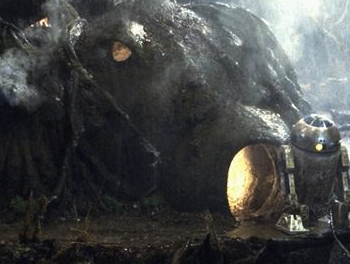
\includegraphics[scale =0.5]{dagobah}@)
;_________________________________________
;Zugriff auf die Liste der Bildpunkte (Pixel) eines Bildes: 
 
;(: image->color-list (image -> (list-of rgb-color)))  
;(: color-list->bitmap ((list-of rgb-color) natural natural -> image))
 
;Breite/Höhe eines Bildes in Pixeln:
 
;(: image-width (image -> natural))
; (: image-height (image -> natural))
 
; Eine Farbe (rgb-color) besteht aus ihrem
; - Rot-Anteil 0..255 (red)
; - Grün-Anteil 0..255 (green)
; - Blau-Anteil 0..255 (blue)

 @
\includegraphics[scale=0.5]{pixel}@
 
; (define-record-procedures rgb-color
;   make-color
;   color?
;   (color-red color-green color-blue))
;________________________________________

; Signatur für color-Records nicht in image2.rkt eingebaut.  Roll our own...
(define rgb-color
  (signature (predicate color?)))


; Ist Farbe c bläulich?
(: bluish? (rgb-color -> boolean))
(define bluish?
  (lambda (c)
    (< (/ (+ (color-red c) (color-green c) (color-blue c))
          3)
       (color-blue c))))

; Worker:
; Pixel aus Hintergrund bg scheint durch, wenn der
; entsprechende Pixel im Vordergrund fg bläulich ist.
; Arbeite die Pixellisten von fg und bg synchron ab
; Annahme: fg und bg haben identische Länge!
(: bluescreen ((list-of rgb-color) (list-of rgb-color) -> (list-of rgb-color)))
(define bluescreen
  (lambda (fg bg)
    (cond ((empty? fg)
           empty)
          ((pair? fg)
           (make-pair 
            (if (bluish? (first fg))
                (first bg)
                (first fg))
            (bluescreen (rest fg) (rest bg)))))))

; Wrapper:
; Mische Vordergrund fg und Hintergrund bg nach Bluescreen-Verfahren
(: mix (image image -> image))
(define mix
  (lambda (fg bg)
    (let ((fg-h (image-height fg))
          (fg-w (image-width fg))
          (bg-h (image-height bg))
          (bg-w (image-width bg)))
      (if (and (= fg-h bg-h)
               (= fg-w bg-w))
          (color-list->bitmap
           (bluescreen (image->color-list fg)
                       (image->color-list bg))
           fg-w
           fg-h)
          (violation "Dimensionen von Vorder-/Hintergrund verschieden")))))

; Yoda vor seine Hüte auf Dagobah setzen
(mix yoda dagobah) @\eval \ 
\includegraphics[scale=0.5]{Yoda_finished}@
\end{filecontents*}
\begin{filecontents*}{notquiteall.rkt}
; Eigenschaft nur auswerten, wenn n > 0 (==>)
(check-property
 (for-all ((n natural))
   (==> (> n 0)   
        (= (succ (pred n)) n))))
\end{filecontents*}
\begin{filecontents*}{Fakultaet.rkt}
; Berechne n!
(: factorial (natural -> natural))
(check-expect (factorial 0) 1)
(check-expect (factorial 3) 6)
(check-expect (factorial 10) 3628800)

(define factorial
  (lambda (n)
    (cond ((= n 0) 1)
          ((> n 0) (* n (factorial (- n 1)))))))
\end{filecontents*}
\begin{filecontents*}{FehlerRekursiv.rkt}
; Fehlerhaft: kein Fortschritt im rekursiven Aufruf
; => potentiell "unendliche" Reduktion
(define unfactorial
  (lambda (n)
    (cond ((= n 0) 1)
          ((> n 0) (* n (unfactorial n))))))

; Fehlerhaft: kein definierter Abbruch der Rekursion
; => Abbruch der Reduktion bei n = 0 ("cond: alle Tests ergaben #f")
(define not-factorial
  (lambda (n)
    (cond ((> n 0) (* n (not-factorial (- n 1)))))))
\end{filecontents*}
\begin{filecontents*}{Endrekursion.rkt}
;; Die ersten drei Zeilen dieser Datei wurden von DrRacket eingefügt. Sie enthalten Metadaten
;; über die Sprachebene dieser Datei in einer Form, die DrRacket verarbeiten kann.
#reader(lib "DMdA-vanilla-reader.ss" "deinprogramm")((modname definitions) (read-case-sensitive #f) (teachpacks ((lib "image2.ss" "teachpack" "deinprogramm"))) (deinprogramm-settings #(#f write repeating-decimal #f #t none explicit #f ((lib "image2.ss" "teachpack" "deinprogramm")))))
; Messung der Reduktionszeit (in Millisekunden) 
; für Ausdruck <e> mittels (time <e>)
(require racket/base)  


; Erinnerung: Generiere Liste von s bis e
(: from-to (natural natural -> (list-of natural)))
(define from-to
  (lambda (s e)
    (cond ((> s e) empty)
          (else (make-pair s (from-to (+ s 1) e)))))) 


; Erinnerung: konkateniere Listen xs und ys
; (Länge von xs bestimmt Anzahl rekursiver Aufrufe)

(: cat ((list-of %a) (list-of %a) -> (list-of %a)))  
(define cat
  (lambda (xs ys)
    (cond ((empty? xs) 
           ys)
          ((pair? xs)
           (make-pair (first xs)
                      (cat (rest xs) ys))))))

; ------------------------------------------------------------------------------

; Berechne n! (nicht endrekursiv)
(: factorial (natural -> natural))
(define factorial
  (lambda (n)
    (cond ((= n 0) 1)
          ((> n 0) (* n (factorial (- n 1)))))))
;                  ^^^^^^^^^^^^^^^^^^^^^^^^
;        nicht-leerer Kontext (* n ▢ ) des rekursiven Aufrufes
           

(factorial 5)


; Berechne n!
; Wrapper
(: fac (natural -> natural))
(check-expect (fac 0) 1)
(check-expect (fac 3) 6)
(define fac
  (lambda (n)
    (fac-worker n 1)))

; Berechne n! (mit Zwischenergebnis/Akkumulator acc), endrekursiv
; Worker
(define fac-worker
  (lambda (n acc)
    (cond ((= n 0) acc)
          ((> n 0) (fac-worker (- n 1) (* n acc))))))
;                  ^^^^^^^^^^^^^^^^^^^^^^^^^^^^^^
;                  endrekursiver Aufruf (tail call)
;                  siehe Syntaxprüfung (rosa Pfeile)

(fac 5)



; Liste xs umdrehen
; Aufwand: 1/2 × n × (n + 1) Aufrufe von make-pair wenn xs die Länge n hat
(: rev ((list-of %a) -> (list-of %a)))

(check-expect (rev empty) empty)
(check-expect (rev (list 1 2 3 4)) (list 4 3 2 1))

(define rev
  (lambda (xs)
    (cond ((empty? xs) empty)
          ((pair? xs) 
           (cat (rev (rest xs)) (list (first xs)))))))


; Liste xs umdrehen (effiziente Variante)
; Wrapper
(: backwards ((list-of %a) -> (list-of %a)))

(check-expect (backwards empty) empty)
(check-expect (backwards (list 1 2 3 4)) (list 4 3 2 1))

(define backwards
  (lambda (xs)
    
    ; Liste xs umdrehen (mit Akkumulator acc, endrekursiv)
    ; Worker
    ; Aufwand: n Aufrufe von make-pair, wenn xs die Länge n hat
    (letrec ((backwards-worker
              (lambda (xs acc)
                (cond ((empty? xs) acc)
                      ((pair? xs) 
                       (backwards-worker (rest xs) (make-pair (first xs) acc)))))))
      
      (backwards-worker xs empty))))

; NB:
; Benutzt letrec, um die rekursive Worker-Definition lediglich
; lokal zu definieren.


; Performance-Test: Umdrehen einer Liste von n = 1000 Elementen
;
; (1) Führt 1/2 × n × (n + 1) = 500500 Aufrufe von make-pair durch:
(time (rev (from-to 1 1000)))

; (2) Führt n = 1000 Aufrufe von make-pair durch:
(time (backwards (from-to 1 1000)))


; NB:
; backwards ist als Funktion `reverse' in DrRacket verfügbar
\end{filecontents*}
\begin{filecontents*}{HigherOrderProcedures.rkt}
; Ist x ein Element in Liste xs?
(: elem? (number (list-of number) -> boolean))
(define elem?
  (lambda (x xs)
    (cond ((empty? xs) #f)
          ((pair? xs)
           (if (= x (first xs))
               #t
               (elem? x (rest xs)))))))
; Gehört der Film f zu den Prequels (Episode I-III, vor "A New Hope")
(: is-prequel? (film -> boolean))
(define is-prequel?
  (lambda (f)
    (let ((a-new-hope (sw-film 1)))
      (< (film-episode f)
         (film-episode a-new-hope)))))

; Erwähnt der Film f den Todesstern in seinem Opening Crawl?
(: mentions-death-star? (film -> boolean))
(define mentions-death-star?
  (lambda (f)
    ; (string-contains s1 s2) liefert #f oder die Position (0..) des Teilstrings s2 in s1
    (natural? (string-contains (film-opening-crawl f) "DEATH STAR"))))
    
; Kommt Obi-Wan Kenobi im Film f vor?
(: features-kenobi? (film -> boolean))
(define features-kenobi?
  (lambda (f)
    (elem? 10 (film-characters f))))



; Filtere Liste xs nach Elementen, die Prädikat p? erfüllen
; (Prozedur höherer Ordnung: Parameter p? ist selbst eine Funktion)
(: filter ((%a -> boolean) (list-of %a) -> (list-of %a)))
(define filter
  (lambda (p? xs)
    (cond ((empty? xs) empty)
          ((pair? xs)  (if (p? (first xs))
                           (make-pair (first xs)
                                      (filter p? (rest xs)))  
                           (filter p? (rest xs)))))))


; Wird filter mit verschiedenen Prädikaten parameterisiert,
; erhalten wir spezifische Filter:

; NB: Auswertung benötigt eine kurze Zeit durch 
;     Zugriff auf das Star Wars Web-API
(define prequels-films
  (filter is-prequel? (sw-films)))

(define death-star-films
  (filter mentions-death-star? (sw-films)))

(define kenobi-films
  (filter features-kenobi? (sw-films)))



; Falte Liste xs bzgl. z und c.  Spine-Transformation:
; - empty     ~~> z
; - make-pair ~~> c
;
;   +--+--+                             
;   |  |  |                             
;   +--+--+                                 c
;   /     \                                / \ 
; x1      +--+--+                        x1   c
;         |  |  |                            / \  
;         +--+--+   ~~(foldr z c xs)~~>    x2   .
;         /     \                                \
;       x2       .                                c
;                 \                              / \  
;                 +--+--+                      xn   z                   |
;                 |  |  |                         
;                 +--+--+                           
;                 /     \             (c x1 (c x2 (... (c xn z)...)))  
;                xn     empty                        
;
(: foldr (%b (%a %b -> %b) (list-of %a) -> %b))
(define foldr
  (lambda (z c xs)
    (cond ((empty? xs) z)
          ((pair? xs)  (c (first xs) (foldr z c (rest xs)))))))
 

; Listenreduktion via foldr: Summe der Liste xs
(: my-sum ((list-of number) -> number))
(define my-sum
  (lambda (xs)
    (foldr 0 + xs)))

; Listenreduktion via foldr: Produkt der Liste xs
(: my-product ((list-of number) -> number))
(define my-product
  (lambda (xs)
    (foldr 1 * xs)))

; Listenreduktion via foldr: Maximum der Liste xs
(: my-maximum ((list-of number) -> number))
(define my-maximum
  (lambda (xs)
    (foldr -inf.0 max xs)))

; Identität (auf Listen), implementiert via foldr
(: my-id ((list-of %a) -> (list-of %a)))
(define my-id
  (lambda (xs)
    (foldr empty make-pair xs)))
    
; Reimplementation von append via foldr
(: my-append ((list-of %a) (list-of %a) -> (list-of %a)))
(define my-append
  (lambda (xs ys)
    (foldr ys make-pair xs)))

; Reimplementation von map via foldr
(: my-map ((%a -> %b) (list-of %a) -> (list-of %b)))
(define my-map
  (lambda (f xs)
    (foldr empty                                
           (lambda (y ys) (make-pair (f y) ys))  
           xs)))

; Reimplementation von reverse via foldr
(: my-reverse ((list-of %a) -> (list-of %a)))
(define my-reverse
  (lambda (xs)
    (foldr empty                                
           (lambda (y ys) (append ys (list y)))
           xs)))

; Listenreduktion via foldr: Länge der Liste xs
(: my-length ((list-of %a) -> natural))
(define my-length
  (lambda (xs)
    (foldr 0 (lambda (x l) (+ 1 l)) xs)))

; Reimplementation von filter mittels foldr
(: my-filter ((%a -> boolean) (list-of %a) -> (list-of %a)))
(define my-filter
  (lambda (p? xs)
    (foldr empty 
           (lambda (y ys) (if (p? y)
                              (make-pair y ys)
                              ys)) 
           xs)))




\end{filecontents*}
\usepackage{fltpoint}
\usepackage{fourier}
\usepackage{hyperref}
\usepackage[ngerman]{babel}
\usepackage{graphicx} %Bilder einbinden
\usepackage[leqno]{amsmath}
\usepackage{amsfonts,amssymb,amsthm,mathtools} %erweiterte Mathe-Zeichen
\setcounter{secnumdepth}{-2}
\usepackage{fancyhdr}
\usepackage{ifthen}
\usepackage{courier}
\usepackage{blkarray}
\usepackage{listings}
\usepackage{tikz}
\usepackage{color}
\usepackage{enumerate}
\usepackage{marginnote}
\usepackage{multirow,booktabs,bigdelim}
\pagestyle{fancy}
\usepackage{marvosym}
\usepackage{mdframed}
\usepackage{pgfplots}
\usepackage{rotating}
\usetikzlibrary{shapes}
\definecolor{string}{rgb}{0.133,0.545,0.133}
\newcommand{\numrak}[1]{\text{\fbox{\textcolor{string}{#1}}}}
\definecolor{kommentar}{rgb}{0.75,0.49,0.07}
\newcommand{\rackett}[5]{\lstinputlisting[frame=single,caption={[#1]#2},firstline=#4,lastline=#5]{#3.rkt}}
\newcommand{\racket}[3]{\lstinputlisting[frame=single,caption={[#1]#2}]{#3.rkt}}
\newcommand{\latexcode}[1]{\textcolor{kommentar}{#1}}
\usepackage[normalem]{ulem} % [normalem] to set \emph{} to default behaviour (italic instead of underlining)
\usepackage{mdsymbol}
\DeclarePairedDelimiter{\ceil}{\lceil}{\rceil}
\DeclarePairedDelimiter{\floor}{\lfloor}{\rfloor}
\fancyhf{}
%\fancyfoot[RE,LO]{\hyperlink{https://github.com/FinnIckler/SS15-Skripte/tree/master/InfoII}{Link}}
\fancyfoot[LE,RO]{\thepage}
\fancyhead[LE,RO]{Informatik II Thorsten Grust}
\fancyhead[LO,RE]{Skript SS15 Finn Ickler}
\rhead{Informatik II Thorsten Grust}
\lhead{Skript SS15 Finn Ickler}
\renewcommand{\lstlistingname}{Codebeispiel}
\renewcommand{\lstlistlistingname}{Codebeispiele}
\newcommand{\auf}{$\langle$}
\newcommand{\zu}{$\rangle$}
\newcommand{\az}[1]{\langle \text{#1}\rangle}
\newcommand{\eval}{$\longrightsquigarrow$}
\newcommand{\reval}{$\longleftsquigarrow$}
\renewcommand{\i}{\item}
\renewcommand{\t}{\text}
\newcommand{\arge}[1]{\auf $\t{e}_{#1}$\zu}
\newcommand{\argt}[1]{\auf $\t{t}_{#1}$\zu}
\newcommand{\argcomp}[1]{\auf $\t{comp}_{#1}$\zu}
\newcommand{\argid}[1]{\auf $\t{id}_{#1}$\zu}
\newcommand{\argf}[1]{\auf $\t{f}_{#1}$\zu}
\lstset{
  language=Macht der Abstraktion
}
\newcommand*\circled[1]{\tikz[baseline=(char.base)]{\node[shape=circle,draw,inner sep=2pt](char){#1};}}
\author{Finn Ickler}
\title{Informatik II Skript Sommersemester 2015}
\hypersetup{%
    pdfborder = {0 0 0}
}
\begin{document}
	\graphicspath{{./Graphics/}}
\renewcommand{\underline}[1]{\emph{#1}}
\renewcommand{\uline}[1]{\emph{#1}}
\maketitle
\tableofcontents
\lstlistoflistings
\newpage
\section{14.4.2015}
\section*{Scheme}
\underline{A}usdr\"ucke , \underline{A}uswertung und \underline{A}bstraktion\\
\subsection*{Dr Racket}
\fbox{
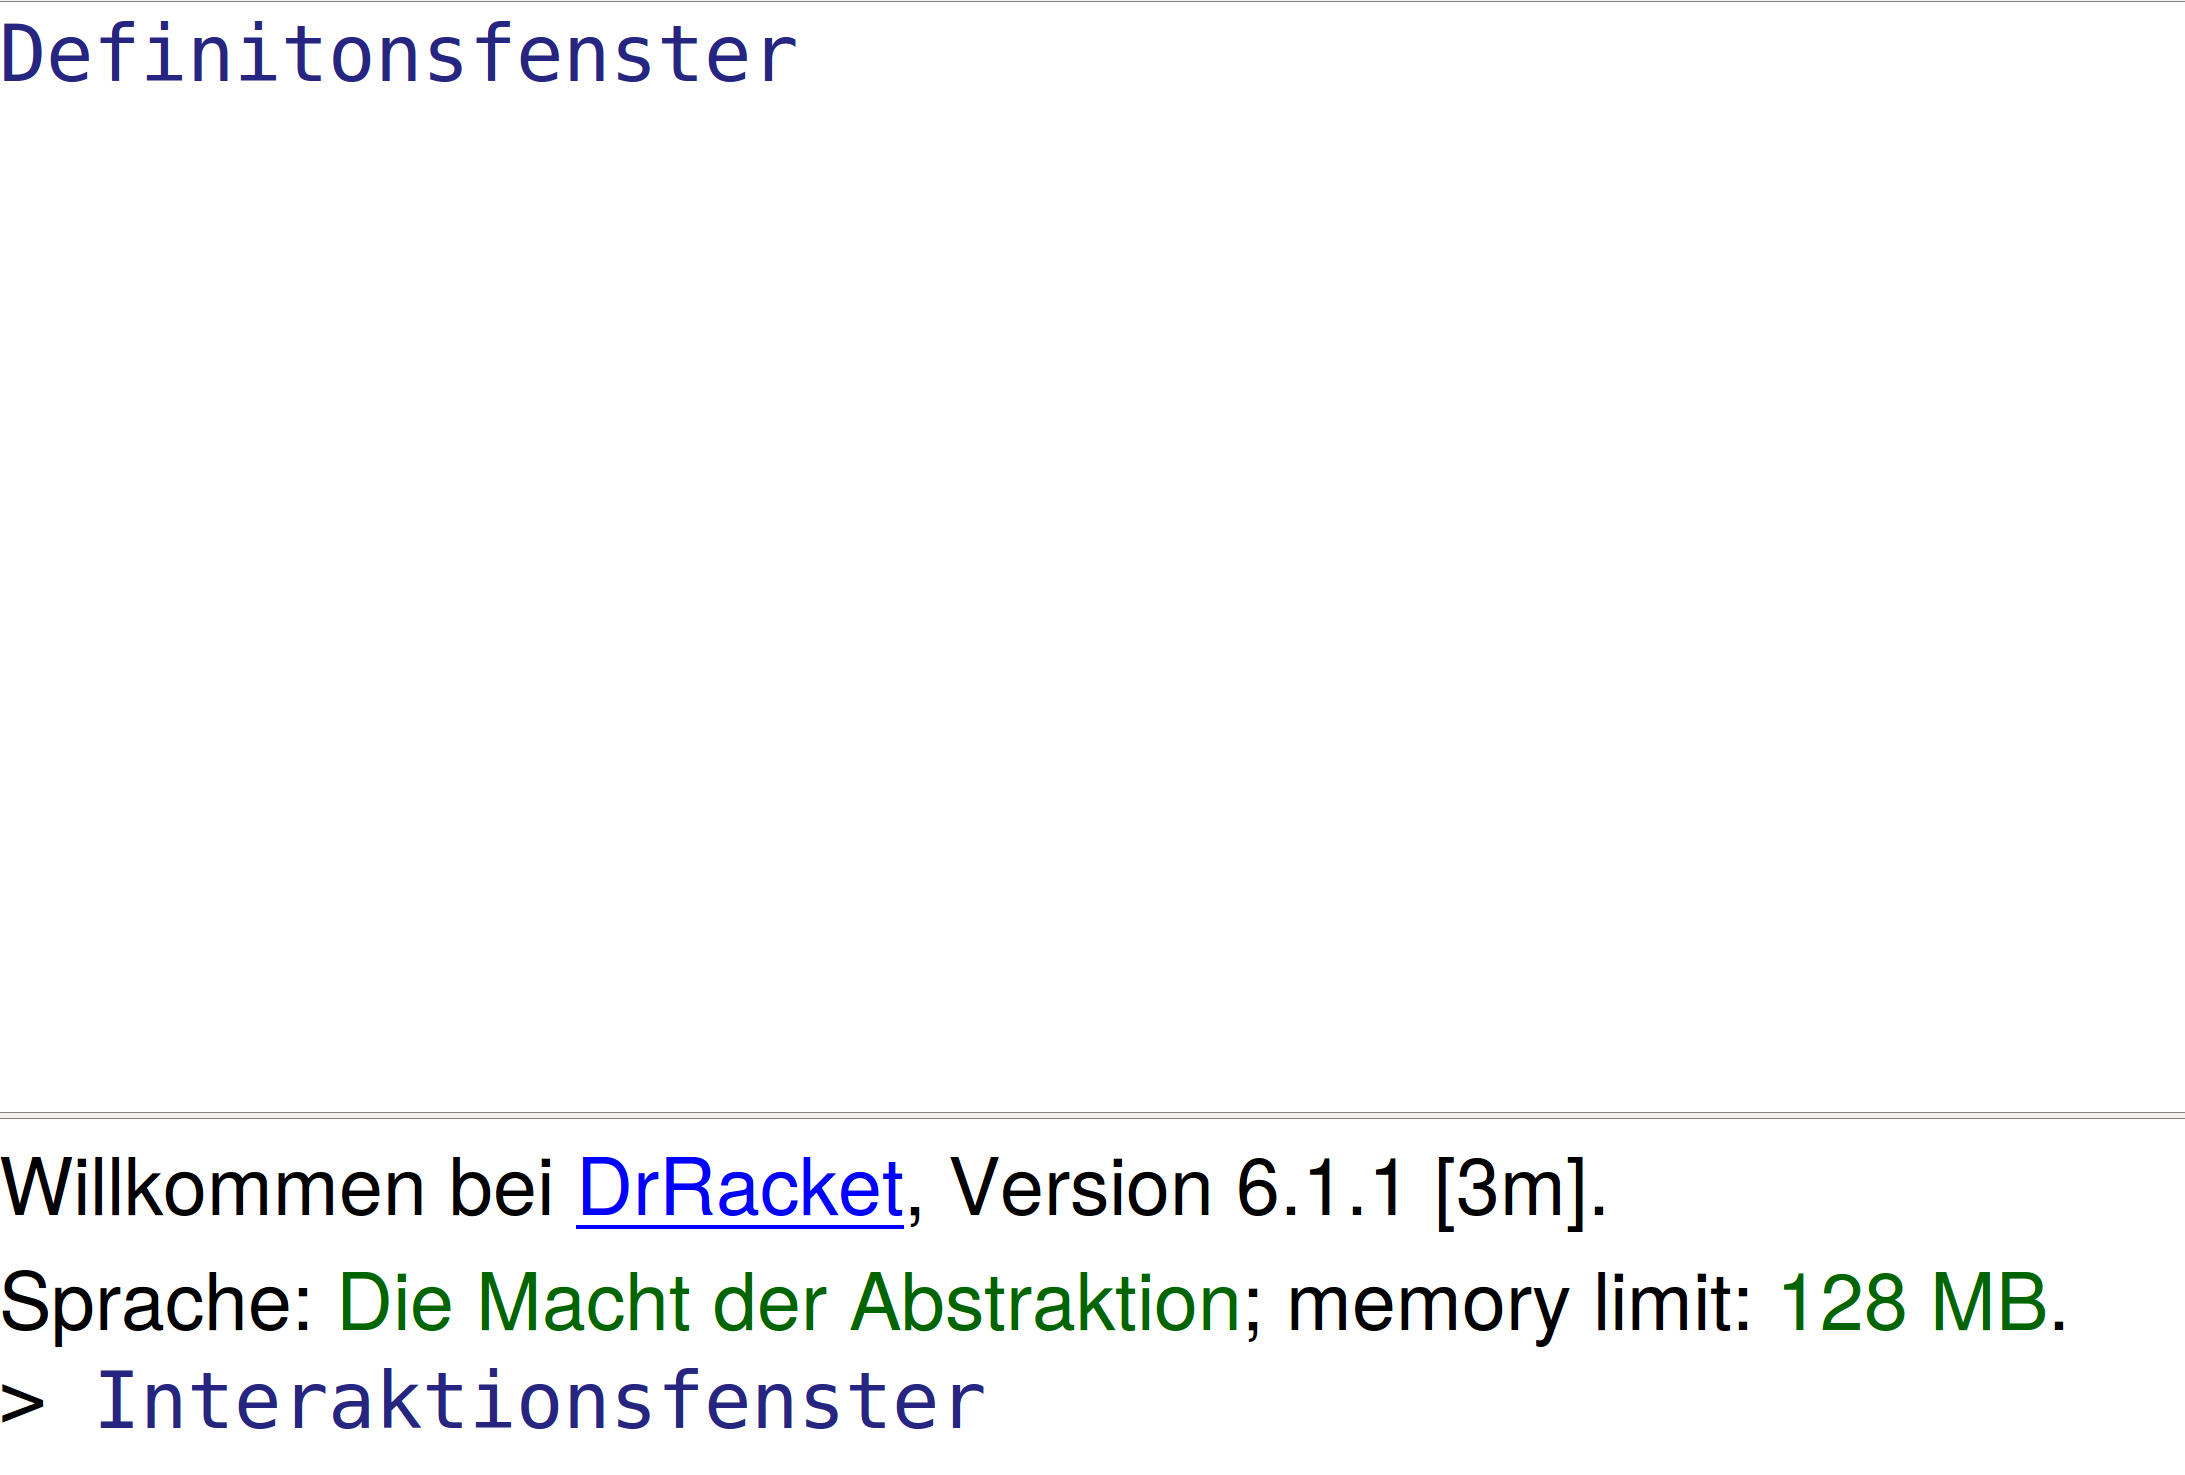
\includegraphics[scale=0.15]{drracket}}\\
Die Anwendung von Funktionen wird in Scheme ausschlie\ss lich in Pr\"afixnotation durchgef\"uhrt
\bigskip\\
\begin{center}
\begin{tabular}{c|c}
Mathematik & Scheme \\
\hline
$44-2$ & $(- $44 2)\\
$f(x,y)$ & (f x y)\\
$\sqrt{81}$ & (sqrt 81)\\
$9^2$ & (expt 92)\\
$3!$ & (! 3)\\
\end{tabular}\\
Allgemein: (\textless funktion\textgreater \textless argument1\textgreater \textless argument2\textgreater \ldots)
\end{center}
(+ 40 2) und (odd? 42) sind Beispiele f\"ur \underline{Ausdr\"ucke}, die bei \underline{Auswertung} einen Wert liefern.\\
(Notation: \eval)\\
(+ 40 2) $\underbrace{\longrightsquigarrow}_{Reduktion}$ 42\\
(odd? 42) \eval \#f
\bigskip\\
Interaktionsfenster:\hspace*{2.5cm} $\underbrace{Read \rightarrow Eval \rightarrow Print \rightarrow Loop}_{REPL}$\\
\bigskip\\
\underline{Literale} sethen f\"ur einen konstanten Wert (auch: \underline{Konstante}) und sind nicht weiter reduzierbar.\\
\begin{center}
\begin{tabular}{ccc}
Literal &  & Sorte,Typ\\
\hline
\#f ,\#t & (true, false, Wahrheitswert) & boolean\\
"x" & (Zeichenketten) & String\\
0 1904 42 $-2$ & (ganze Zahl) & Integer\\
0.42 3.14159 & (Flie\ss kommazahl) & real\\
1\textbackslash 2, 3\textbackslash 4, -1\textbackslash 10 & (rationale Zahlen) & rational\\

\includegraphics[scale=0.2]{Darth_Vader} & (Bilder) & image

\end{tabular}
\end{center}



\section{16.4.2015}

Auswertung \underline{zusammengesetzter Ausdr\"ucke} in mehreren Schritten (Steps), von ``innen nach au\ss en``, bis keine Reduktion mehr m\"oglich ist.\\
\begin{lstlisting}
(+ ( @\uwave{(+ 20 20)}@ (+ 1 1)) @\eval@ (+ 40 @\uwave{(+ 1 1)}@ @\eval@ (+ 40 2) @\eval@  42 
\end{lstlisting}
\rackett{Arithmetik mit Flie\ss kommazahlen}{\textbf{Achtung:} Scheme rundet bei Arithmetik mit Flie\ss kommazahlen (interne Darstellung ist binär}{Grundlagen}{4}{17}
Ein Wert kann an einen \underline{Namen} (auch \underline{Identifier}) gebunden werden, durch \\
\lstinline!(define <id> <e>)! \hspace*{1.5cm} \auf id\zu Identifier \ \auf e\zu Ausdruck\\
Erlaubte konsistente Wiederverwendung, dient der Selbstdokumentation von Programmen\\
\textbf{\underline{Achtung:}} Dies ist eine sogenannte Spezialform und kein Ausdruck. Insbesondere besitzt diese Spezialform \underline{keinen} Wert, sondern einen Effekt Name \auf id\zu \ wird an den \underline{Wert} von \auf e\zu \ gebunden. \\
Namen k\"onnen in Scheme beliebig gewählt werden, solange
\begin{enumerate}
\item[(1)] die Zeichen ( ) $[$ $]$ $\{ \}$ `` , ` ` ; \# $\mid$ \textbackslash nicht vorkommen
\item[(2)] dieser nicht einem numerischen Literal gleicht.
\item[(3)] kein Whitespace (Leerzeichen, Tabulator, Return) enthalten ist.
\end{enumerate}
Beispiel: euro$\rightarrow$US\$\\
\underline{\textbf{Achtung:}} Gro\ss-\textbackslash Kleinschreibung ist irrelevant.
\bigskip\\
\lstinputlisting[frame=single,caption={[Schlüsselwort define]Bindung von Werten an Namen},firstline=19,lastline=24]{Grundlagen.rkt}
Eine \underline{lambda-Abstraktion} (auch Funktion, Prozedur) erlaubt die Formatierung von Ausrdr\"ucken, in denen mittels \underline{Parametern} von konkreten Werten abstrahiert wird.\\
\lstinline[literate=]!(lambda (<p1><p2>...) <e>!\\
\auf e\zu Rumpf: enth\"alt Vorkommen der Parameter \auf $p_n$\zu\\
(lambda($\ldots$)) ist eine Spezialform. Wert der lambda-Abstraktion ist \#\auf procedure\zu\\.
\underline{Anwendung} (auch Application) des lambda-Aufrufs f\"uhrt zur Ersetzung aller Vorkommen der Parameter im Rumpf durch die angegebenen \uline{Argumente}.\\
\lstinputlisting[frame=single,caption={[Lambda Abstraktion] Lambda-Abstraktion},firstline=26,lastline=34]{Grundlagen.rkt}
\lstinline!(lambda (days) (* days (* 155!\lstinline! minutes-in-a-day))) 365)! \eval\\
\lstinline!(* 365 (* 155!\lstinline! minutes-in-a-day))! \eval  \lstinline!81468000!\\
\bigskip\\
In Scheme leitet ein Semikolon einen Kommentar ein, der bis zum Zeilenende reicht und vom System bei der Auswertung ignoriert wird.\\
Prozeduren sollten im Programm ein- bis zweizeilige \underline{Kurzbeschreibungen} direkt vorangestellt werden.
\section{21.4.2015}
Eine Signatur pr\"uft, ob ein Name an einen Wert einer angegebenen Sorte (Typ) gebunden wird. Signaturverletzungen werden protokolliert.\\
\lstinline!(: <id> <signatur>)!\\
Bereits eingebaute Sinaturen\\
\begin{tabular}{rc|r}
natural&$\mathbb{N}$& boolean\\
integer&$\mathbb{Z}$& string\\
rational&$\mathbb{Q}$& image\\
real&$\mathbb{R}$&$\ldots$\\
number&$\mathbb{C}$
\end{tabular}\\
\lstinline!(: ...)! ist eine Spezialform und hat keinen Wert, aber einen Effekt: Signaturpr\"ufung\\
\uline{Prozedur Signatur} spezifizieren sowohl Signaturen f\"ur die Parameter $\text{P}_1,\text{P}_2,\ldots\text{P}_n$ als auch den Ergebniswert der Prozedur,\\
\lstinline[literate=]!(: <Signatur P1> ... <Signatur Pn> -> <Signatur Ergebnis>)!\\
Prozedur Signaturen werden \underline{bei jeder Anwendung} einer Prozedur auf Verletzung gepr\"uft. \underline{Testf\"alle} dokumentieren das erwartete Ergebnis einer Prozedur f\"ur ausgew\"ahlte Argumente:
\begin{center}
\lstinline[literate=]!(check-expect <e1> <e2>)!\end{center}
Werte Ausdruck \auf $\text{e}_1$\zu \ aus und teste, ob der erhaltene Wert der Erwartung \auf $\text{e}_2$\zu \ entspricht (= der Wert von \auf $\text{e}_2$\zu) \
Einer Prozedur sollte Testf\"alle direkt vorangestellt werden.\\
Spezialform: kein Wert, sondern Effekt: Testverletzung protokollieren
\bigskip\\
\underline{Konstruktionsanleitung f\"ur Prozeduren:}
\begin{enumerate}
\item[(1)]Kurzbeschreibung (ein- bis zweizeiliger Kommentar mit Bezug auf Parametername)
\item[(2)]Signaturen
\item[(3)]Testf\"alle
\item[(4)]Prozedurrumpf
\end{enumerate}
\underline{Top-Down-Entwurf} (Programmieren durch ``Wunschdenken``)\\
Beispiel: Zeichne Ziffernblatt (Stunden- und Minutenzeiger) zu Uhrzeit h:m auf einer analogen 24h-Uhr\\
\begin{tikzpicture}
    \begin{axis}[
    legend style={draw none},
    axis equal,ymin = -2,xmin = -2,ymax = 2,
    xmax = 2,xtick ={},
    hide axis,
    xticklabels={},
    ytick ={},
    yticklabels={},
    extra x ticks={0},
    extra x tick label={},
    extra y ticks={0},
    extra y tick labels={},
    disabledatascaling,
    extra tick style = {grid = major}]
    \draw (axis cs:0,0) circle[radius=1];
    \draw[->](axis cs:0,0)--(axis cs:0.64,0.5);
    \draw[->](axis cs:0,0)--(axis cs:0.4,0);
    \end{axis}   
  \end{tikzpicture}\\
  Minutenzeiger legt $\frac{360^{\circ}}{60}$ Grad pro Minute zur\"uck (also $\frac{360}{60} \cdot m$)\\
  Studentenzeiger legt $\frac{360}{12}$ pro Stunde zur\"uck
 ($\frac{360}{12} \cdot h +\frac{360}{12} \cdot \frac{m}{60}$)
 \rackett{Bilderzusammenstellung am Beispiel einer Uhr}{Bauen der Uhr durch Top Down Entwurf}{Uhr}{4}{45}

\section{23.4.2015}
\underline{Substitutionsmodell}\\
\underline{Reduktionsregeln} f\"ur Scheme (Fallunterscheidung je nach Ausdr\"ucken) wiederhole, bis keine Reduktion mehr m\"oglich\\
\begin{tabular}{llc}
$-$literal (1, ``abc``, $\#$t, $\ldots$)& l \eval l &$[\text{eval}_{lit}]$\\
$-$Identifier id(pi, clock-face,$\ldots$)& id \eval gebundene Wert& $[\text{eval}_{id}]$\\
$-$lambda Abstraktion &(lambda ($\ldots ) \ldots$) \eval lamba($\ldots) \ldots)$ & $[\text{eval}_{\lambda}]$\\
$-$Applikationen (f $e_1$ $e_2 \ldots$)\\
\end{tabular}
\begin{equation}
f,e_1,e_2 \text{ reduzieren erhalte:} f`,e_1`,e_2`\\
\end{equation}\\
(2)
$\begin{cases}
\text{Operation }f`\text{ auf }e_1` \text{ und } e_2` \ [\text{apply}_{prim}] &\mbox{falls } f`\text{ primitiv ist}\\
\text{Argumentenwerte in den Rumpf von} f`\text{ einsetzen, dann reduzieren }&\mbox{falls } f`\text{ lambda Abstraktion}
\end{cases}$
\bigskip\\
Beispiel:\\
(+ 40 2) $\text{\eval}_{eval id}$ (\# \auf procedure +\zu 40 2) \eval 42
\bigskip\\
\begin{tabular}{lll}
(position-minute-hand 30) &$\underset{\t{eval id}}{\t{\eval}}$& ((lambda (m) (* degrees-per-minute m)) 30)\\
&$\underset{\t{eval lambda}}{\t{\eval}}$&(* degrees-per-minute 30)\\
&$\underset{\t{eval id}}{\t{\eval}}$&(\# \auf procedure *\zu $\frac{360}{60}$ 30)\\
&$\underset{\t{apply prim}}{\t{\eval}}$&180\\
\end{tabular}\\
Bezeichnen (lambda (x) (* x x)) und lambda (r) (* r r) die gleiche Prozedur? $\Rightarrow$ JA!\\
Achtung: Das hat Einflu\ss \ auf das Korrekte Einsetzen von Argumenten f\"ur Prozeduren (siehe apply)
\bigskip\\
\section*{Prinzip der Lexikalischen Bindung}
Das \underline{bindene Vorkommen} eines Identifiers id kann im Programmtext systematisch bestimmt werden: Suche strikt von innen nach au\ss en, bis zum ersten
\begin{enumerate}[(1)]
\i (lambda (r) \auf Rumpf\zu
\i (define \auf e\zu)
\end{enumerate}
\"Ubliche Notation in der Mathematik: \underline{Fallunterscheidung}\\
$max(x_1,x_2) =
\begin{cases}
x_1 &\text{ falls } x_1 \geq x_2\\
x_2 &\text{ sonst } 
\end{cases}$\\
\underline{Tests} (auch Pr\"adikate) sind Funktionen, die einen Wert der Signatur boolean liefern. Typische primitive Tests.\\
(: = (number number -> boolean))\\
(: \auf (real real -> boolean))\\
auch $>,<=,>=$\\
(: String=? (string string -> boolean))\\
auch string$>$?, string$<=?$\\
(: zero? (number -> boolean))\\
odd?,even?,positive?,negative?\\
Bin\"are Fallunterscheidung \underline{if}\\
$\begin{array}{lcl}
if\\
& <e_1>& \t{Mathematik:}\\
& <e_2>& \begin{cases}e_1& \t{falls } t_1\\
					  e_2& \t{sonst}
\end{cases}\\
& <e_2>)
\end{array}$




\section{28.4.2015}
Die Signatur \underline{one of} lässt genau einen der ausgewählten Werte zu.\\
\lstinline[mathescape]!(one of <$e_1$> <$e_2$> ... <$e_n$>)!\\
\rackett{Die one-of Signatur}{one-of am Beispiel des Fu\ss ballpunktesystems}{Prozeduren}{242}{251}
Reduktion von if:\\
\lstinline[mathescape]!(if $t_1$ <$e_1$> <$e_2$>)!\\
\circled{1} Reduziere $t_1$, erhalte $t_1'$ $\underset{\text{\circled{2}}}{\text{\eval}}
\begin{cases}
\t{\arge{1}} &\t{falls } t_1' = \t{\lstinline!#t!}, \t{\arge{2} niemals ausgewertet}\\
\t{\arge{2}} &\t{falls } t_1' = \t{\lstinline!#f!}, \t{\arge{1} niemals ausgewertet}  
\end{cases}$\\
\rackett{Konstruktion eines eigenen Ifs?}{Koennen wir unser eigenes `if' aus `cond' konstruieren?  (Nein!)}{Prozeduren}{257}{277}
Spezifikation Fallunterscheidung (conditional expression):\\
\begin{tabular}{rlcl}
\lstinline!(cond!& & & Mathematik:\\
&\lstinline[mathescape]!(<$t_1$> <$e_1$>)!&\rdelim\{{5}{0mm}
[] &$e_1$ falls $t_1$ \\
&\lstinline[mathescape]!(<$t_2$> <$e_2$>)!& &$e_2$ falls $t_2$]\\
&\lstinline[mathescape]!$\ldots$!& & $\ldots$\\
&\lstinline[mathescape]!(<$t_n$> <$e_n$>)! & &$e_n$ falls $t_n$\\
&\lstinline[mathescape]!(else <$e_{n+1}$>))! & & $e_{n+1}$ sonst
\end{tabular}\\
Werte die Tests in den Reihenfolge $t_1,t_2.t_3,\ldots,t_n$ aus.\\
Sobald $t_i \#t$ ergibt, werte Zweig $e_i$ aus. $e_i$ ist Ergebnis der Fallunterscheidung. Wenn $t_n \#t$ liefert, dann liefert $\\
\begin{cases}
\t{Fehlermeldung \glqq \textcolor{red}{cond: alle Tests ergaben false}\grqq}& \t{falls kein else Zweig}\\
\text{\lstinline[mathescape]!$\t{\arge{n+1}}$!}& \t{sonst}
\end{cases}$
\newpage
\rackett{Absolutbetrag durch cond}{Absolutwert von x}{Prozeduren}{228}{234}
Reduktion von cond $\lbrack \t{eval}_{\t{cond}}\rbrack $\\
\lstinline[mathescape]!(cond (<$t_1$> <$e_1$>)(<$t_2$> <$e_2$>)$\ldots$(<$t_n$> <$e_n$>))!\\
\circled{1} Reduziere $t_1$ erhalte $t_1'$ $\underset{\t{\circled{2}}}{\t{\eval}} \begin{cases}
\t{\lstinline[mathescape]!<e_1>!} & \t{falls }t_1' = \t{\lstinline!#t!}\\
(\t{\lstinline[mathescape]!cond <t_2> <e_2>)!} & \t{sonst}
\end{cases}$\\
\lstinline[mathescape]!(cond)! \eval \glqq Fehlermeldung : \textcolor{red}{alle Test ergaben false} \grqq\\
\lstinline[mathescape]!(cond (else <$e_{n+1}$>))! \eval $e_{n+1}$\\
\bigskip\\
cond ist syntaktisches Zucker (auch abgeleitete Form) für eine verbundene Anwendung von if \\
\begin{lstlisting}[literate=]
(cond 	(<t1><e1>) 		if (<t1>
	(<t2><e2>)	    	    <e1>
	...				if <t2>
	...				if <e2>
	...				...
	(<tn><en>)       	    	  if <tn>
					     <en>
	(else <en+1>)  	 			<en+1>))..))
\end{lstlisting}
Spezialform 'and' und 'or' \\
\lstinline[mathescape]!(or $\t{\argt{1}}$ $\t{\argt{2}}$ $\ldots$ $\t{\argt{n}}$)! \eval \lstinline[mathescape]!(if $\t{\argt{1}}$ (or $\t{\argt{2}}$ $\ldots$ $\t{\argt{n}}$) #t)!\\
\lstinline[mathescape]!(or)! \eval \lstinline[mathescape]!#f! \\
\lstinline[mathescape]!(and $\t{\argt{1}}$ $\t{\argt{2}}$ $\ldots$ $\t{\argt{n}}$)! \eval \lstinline[mathescape]!(if $\t{\argt{1}}$ (and $\t{\argt{2}}$ $\ldots$ $\t{\argt{n})}$ #f)!\\
\lstinline[mathescape]!(and)! \eval \lstinline[mathescape]!#t!
\newpage
\rackett{Boolsche Ausdrücke mit and und or}{Konstruktion komplexer Prädikate mittels `and' und `or'}{Prozeduren}{281}{296}

\section{30.4.2015}
\underline{Zusammengesetze Daten}\\
Ein Charakter \underline{besteht} aus drei \underline{Komponenten}\\
\begin{tabular}{clcl}
- & Name des Charakters &(name)\rdelim\}{3}{0mm}
[Datendefinition für zusammengesetzte Daten]\\
- & Handelt es sich um einen Jedi? &(jedi?)&\\
- & Stärke der Macht \hspace*{2.3cm} &(force)&
\end{tabular}\\
Konkrete Charakter:\hspace*{5pt}
\begin{tabular}{|c|c|}
\hline
name & \glqq Luke Skywalker \grqq\\
\hline
jedi? & \#f \\
\hline
force & 25 \\
\hline
\end{tabular}\\
\begin{lstlisting}[frame=listing]
; Ein Charakter (character) besteht aus
; - Name (name)
; - Jedi-Status (jedi?)
; - Stärke der Macht (force)
(: make-character (string boolean real -> character))
(: character? (any -> boolean))
(: character-name (character -> string))
(: character-jedi? (character -> boolean))
(: character-force (character -> real))
(define-record-procedures character
  make-character
  character?
  (character-name
   character-jedi?
   character-force))

; Definiere verschiedene Charaktere des Star Wars Universums
(define luke
  (make-character "Luke Skywalker" #f 25))
(define r2d2
  (make-character "R2D2" #f 0))
(define dooku
  (make-character "Count Dooku" #f 80))
(define yoda
  (make-character "Yoda" #t 85))

\end{lstlisting}
Zusammengesetzte Daten = \underline{Records} in Scheme Record-Definition legt fest:\\
\begin{tabular}{cll}
- & Record-Signatur\\
- & \underline{Konstruktor} & (baut aus Komponenten einen Record)\\
- & Prädikat & (liegt ein Record vor?)\\
- & Liste von \underline{Selektoren}& (lesen jeweils eine Komponente des Records)
\end{tabular}\\
\begin{lstlisting}
(define-record-procedure <t>
	make-<t>
	<t>?
	(<t>-<comp1> ... <t>-<comp2>))
	;Liste der n Selektoren
\end{lstlisting}
Verträge des Konstruktors\/ der Selektoren für Record- Signatur\\
\argt{} mit Komponenten namens \argcomp{1} $\ldots$ \argcomp{n}\\
\begin{lstlisting}
(: make-<t> (<t1>...<t2>) -> <t>)
(: <t>-<comp1> (<t> -> <t1>))
(: <t>-<compn> (<t> -> <tn>))
\end{lstlisting}
Es gilt für alle Strings n, Booleans j und Integer f:
\begin{lstlisting}
(character-name (make-character n j f) n)
(character-jedi? (make-character n j f) j)
(character-force (make-character n j f) f )
\end{lstlisting}
Spezialform check-property:\\
\begin{lstlisting}
(check-property
	(for-all ((<id1> <sig1>) ... 
			  (<idn> <sign>))
	<e>))
	@\latexcode{$\downarrow$}@
;Bezieht sich auf <id1> ... <idn>	
\end{lstlisting}
Test erfolgreich, falls \arge{} für beliebig gewählte Bedeutungen für \argid{1} $\ldots$ \argid{n} immer \#t ergibt\\
Interaktion von Selektoren und Konstruktor:
\begin{lstlisting}[frame=listing]
(check-property 
 (for-all ((n string)
           (j boolean)
           (f real))
   (expect (character-name (make-character n j f)) n)))

(check-property 
 (for-all ((n string)
           (j boolean)
           (f real))
   (expect (character-jedi? (make-character n j f)) j)))

(check-property 
 (for-all ((n string)
           (j boolean)
           (f real))
   (expect-within (character-force (make-character n j f)) f 0.001)))
\end{lstlisting}
\underline{Beispiel:} Die Summe von zwei natürlichen Zahlen ist mindestens so gro\ss \ wie jeder dieser Zahlen: $ \forall x_1 \in \mathbb{N}, x_2 \in \mathbb{N} : x_1 + x_2 \geq \max\{x_1,x_2\}$
\begin{lstlisting}[frame=single]
; Für alle natürlichen Zahlen x1,x2 gilt: x1 + x2 @$\textcolor{kommentar}{\geq}$@ max(x1,x2)
(check-property
 (for-all ((x1 natural)
           (x2 natural))
   (>= (+ x1 x2) (max x1 x2))))
\end{lstlisting}
Konstruktion von Funktionen, die bestimmte gesetzte Daten \underline{konsumiert}.\\
\begin{enumerate}[-]
\i Welche Record-Componenten sind relevant für Funktionen?
\begin{enumerate}[$\rightarrow$]
\i Schablone:
\begin{lstlisting}
(: sith? (character -> boolean))
(define sith?
  (lambda (c)
    ... (character-jedi? c))
    ... (character-force c) )...))
\end{lstlisting}
\end{enumerate}
Konstruktion von Funktionen, die zusammengesetzte Daten \underline{konstruieren}
\i Der konstruktor \underline{muss} aufgerufen werden
\begin{enumerate}[$\rightarrow$]
\i Schablone:
\begin{lstlisting}
(define
	lambda(...)
		... (make-<t>)...)
\end{lstlisting}
\end{enumerate}
\i Konkrete Beispiele:
\begin{lstlisting}[frame=single]
; Könnte Charakter c ein Sith sein?
(: sith? (character -> boolean))
(check-expect (sith? yoda) #f)
(check-expect (sith? r2d2) #f)
(define sith?
  (lambda (c)
    (and (not (character-jedi? c))
         (> (character-force c) 0))))


; Bilde den Charakter c zum Jedi aus (sofern c überhaupt Macht besitzt)
(: train-jedi (character -> character))

(check-expect (train-jedi luke) (make-character "Luke Skywalker" #t 50))
(check-expect (train-jedi r2d2) r2d2)

(define train-jedi
  (lambda (c)
    (make-character (character-name c) 
                    (> (character-force c) 0)
                    (* 2 (character-force c)))))
\end{lstlisting}
\end{enumerate}

\section{5.5.2015}
\begin{tikzpicture}[
    grow=right,
    level 1/.style={sibling distance=3.5cm,level distance=5.2cm},
    level 2/.style={sibling distance=3.5cm, level distance=6.7cm},
    edge from parent/.style={very thick,draw=blue!40!black!60,
        shorten >=5pt, shorten <=5pt},
    edge from parent path={(\tikzparentnode.east) -- (\tikzchildnode.west)},
    kant/.style={text width=2cm, text centered, sloped},
    every node/.style={text ragged, inner sep=2mm},
    punkt/.style={rectangle, rounded corners, shade, top color=white,
    bottom color=blue!50!black!20, draw=blue!40!black!60, very
    thick }
    ]

\node[punkt, text width=5.5em] {lego-character}
    %Lower part lv1
    child {
        node[punkt] [rectangle split, rectangle split, rectangle split parts=4,
         text ragged] {
            \textbf{character}
                  \nodepart{second}
            name
                  \nodepart{third}
            jedi?
            	  \nodepart{fourth}
            force	  
        }
        edge from parent
            node[kant, below, pos=.6] {}
    }
    %Upper part, lv1
    child {
        node[punkt, text width=6em] {Figure}
        %child 2
            edge from parent{
                node[kant, above] {}}
    };
\end{tikzpicture}\\
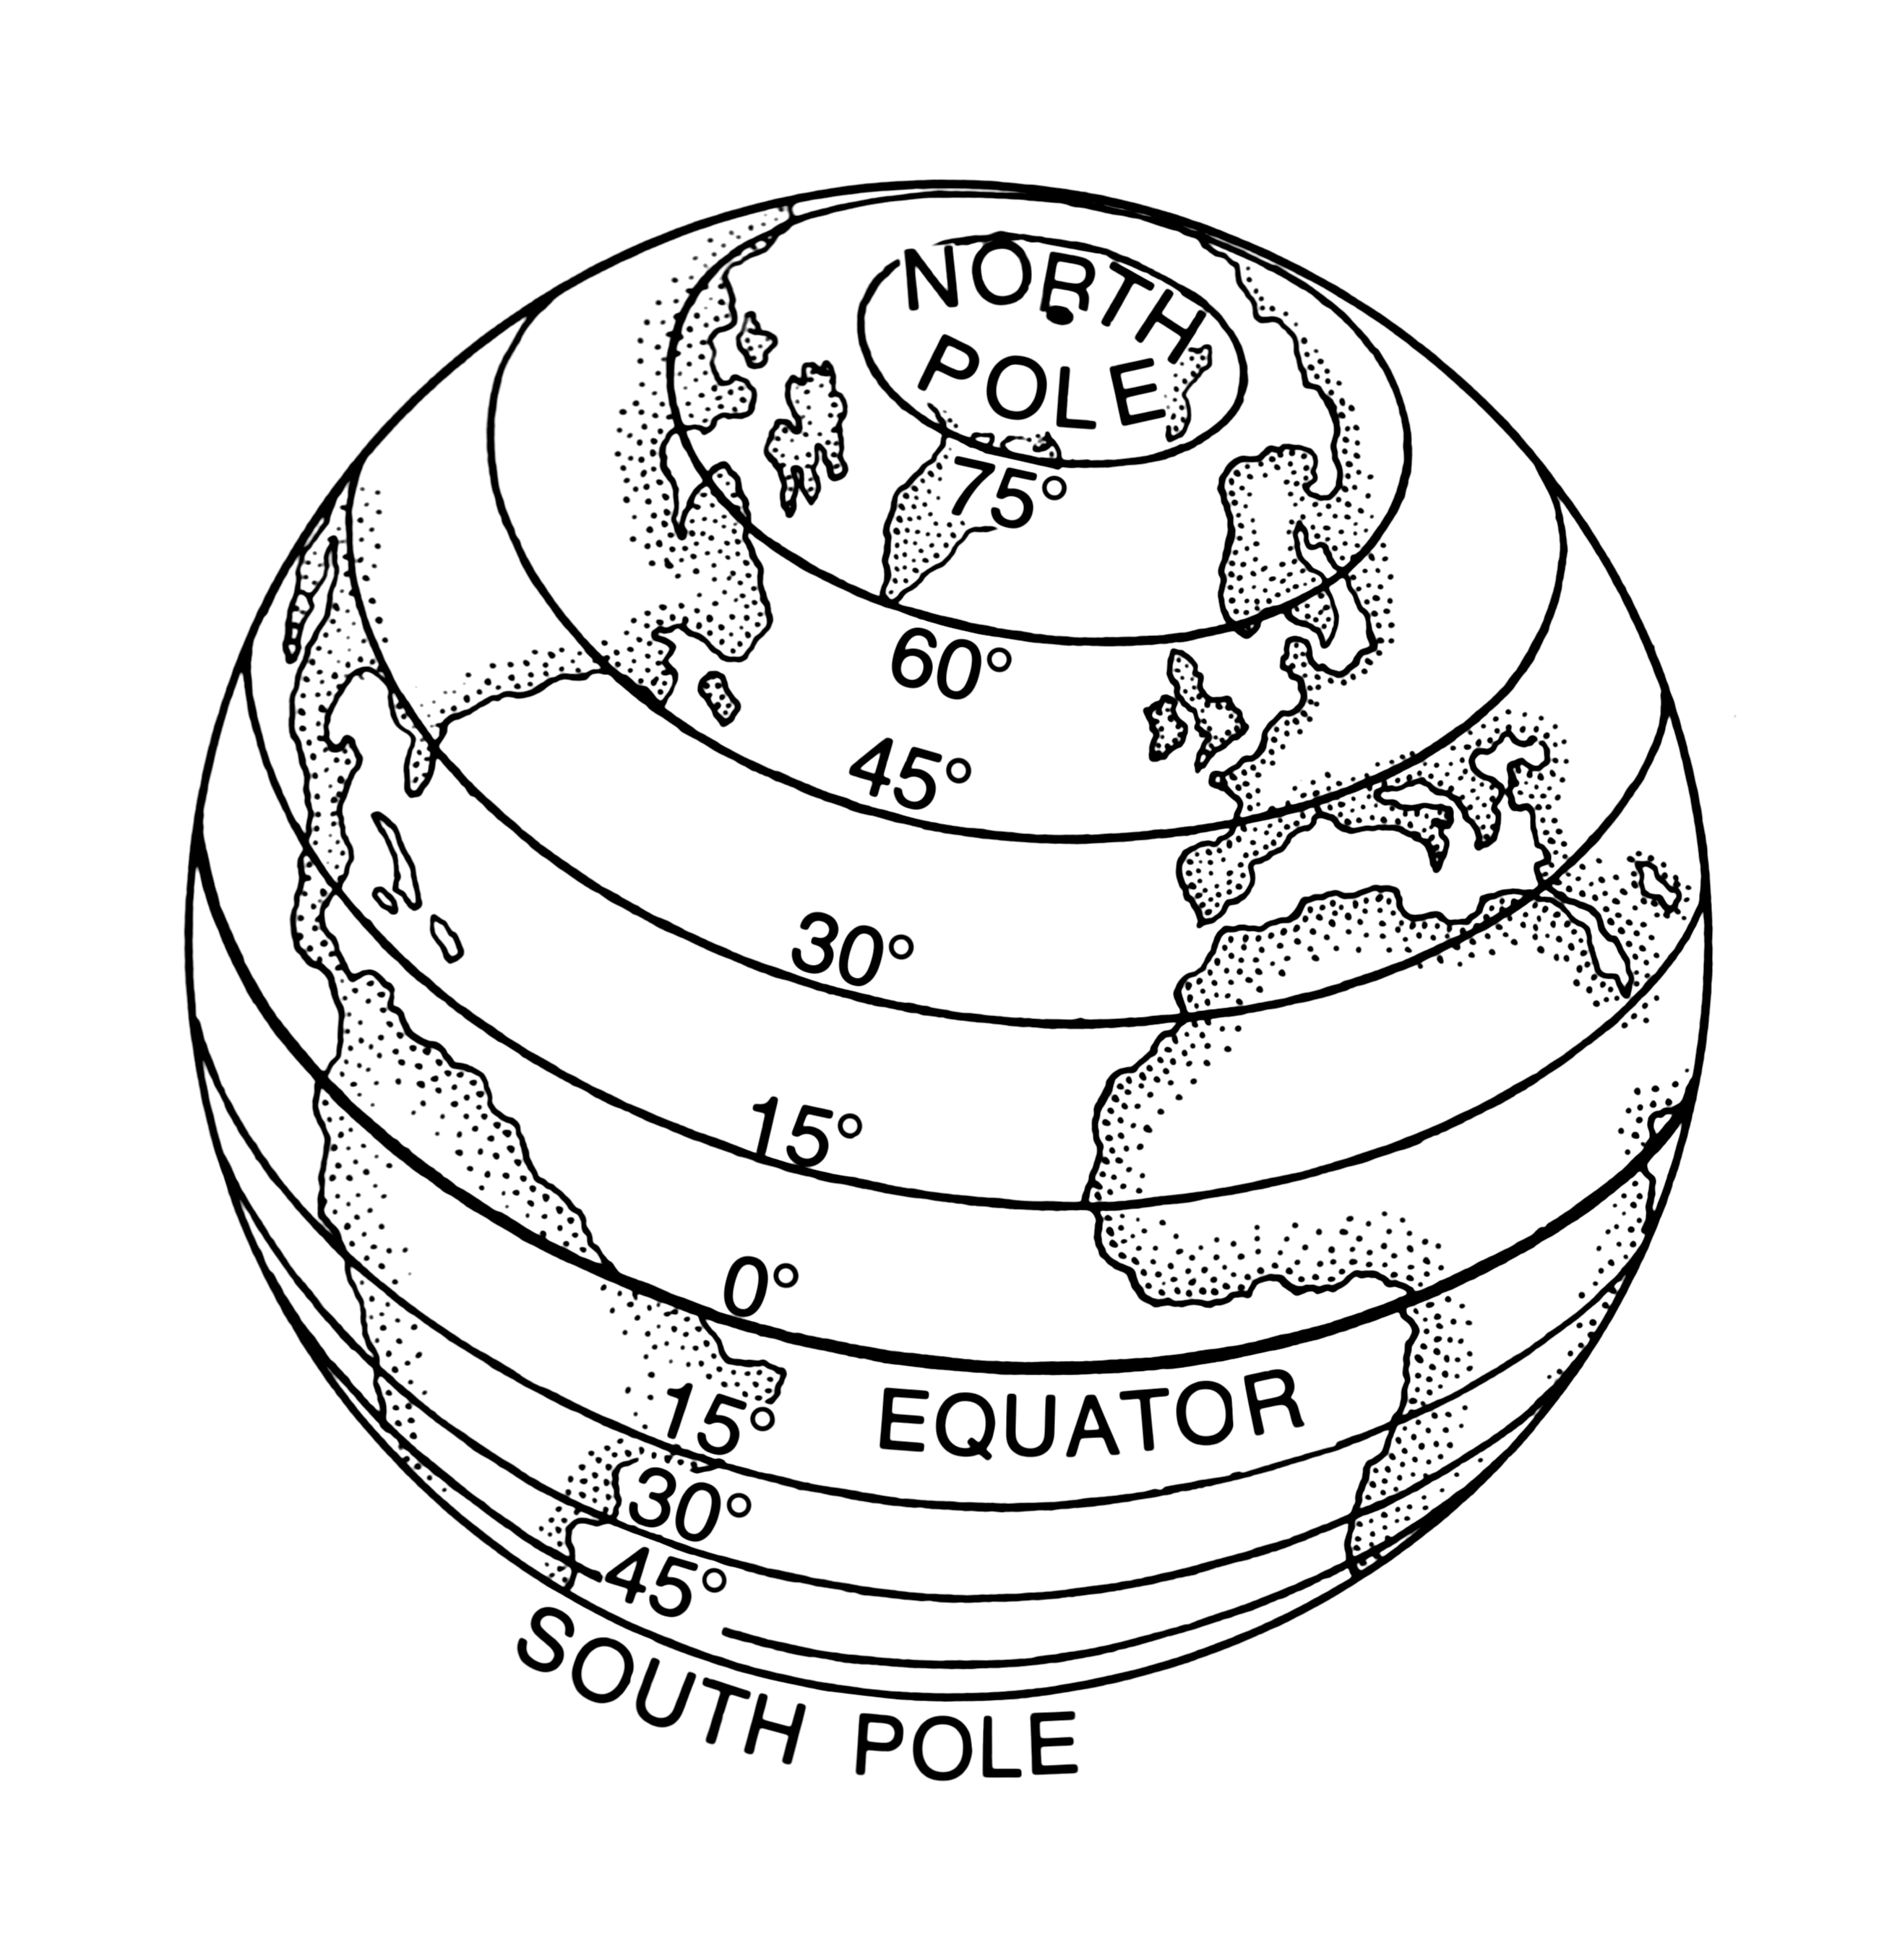
\includegraphics[scale=0.5]{Latitude}
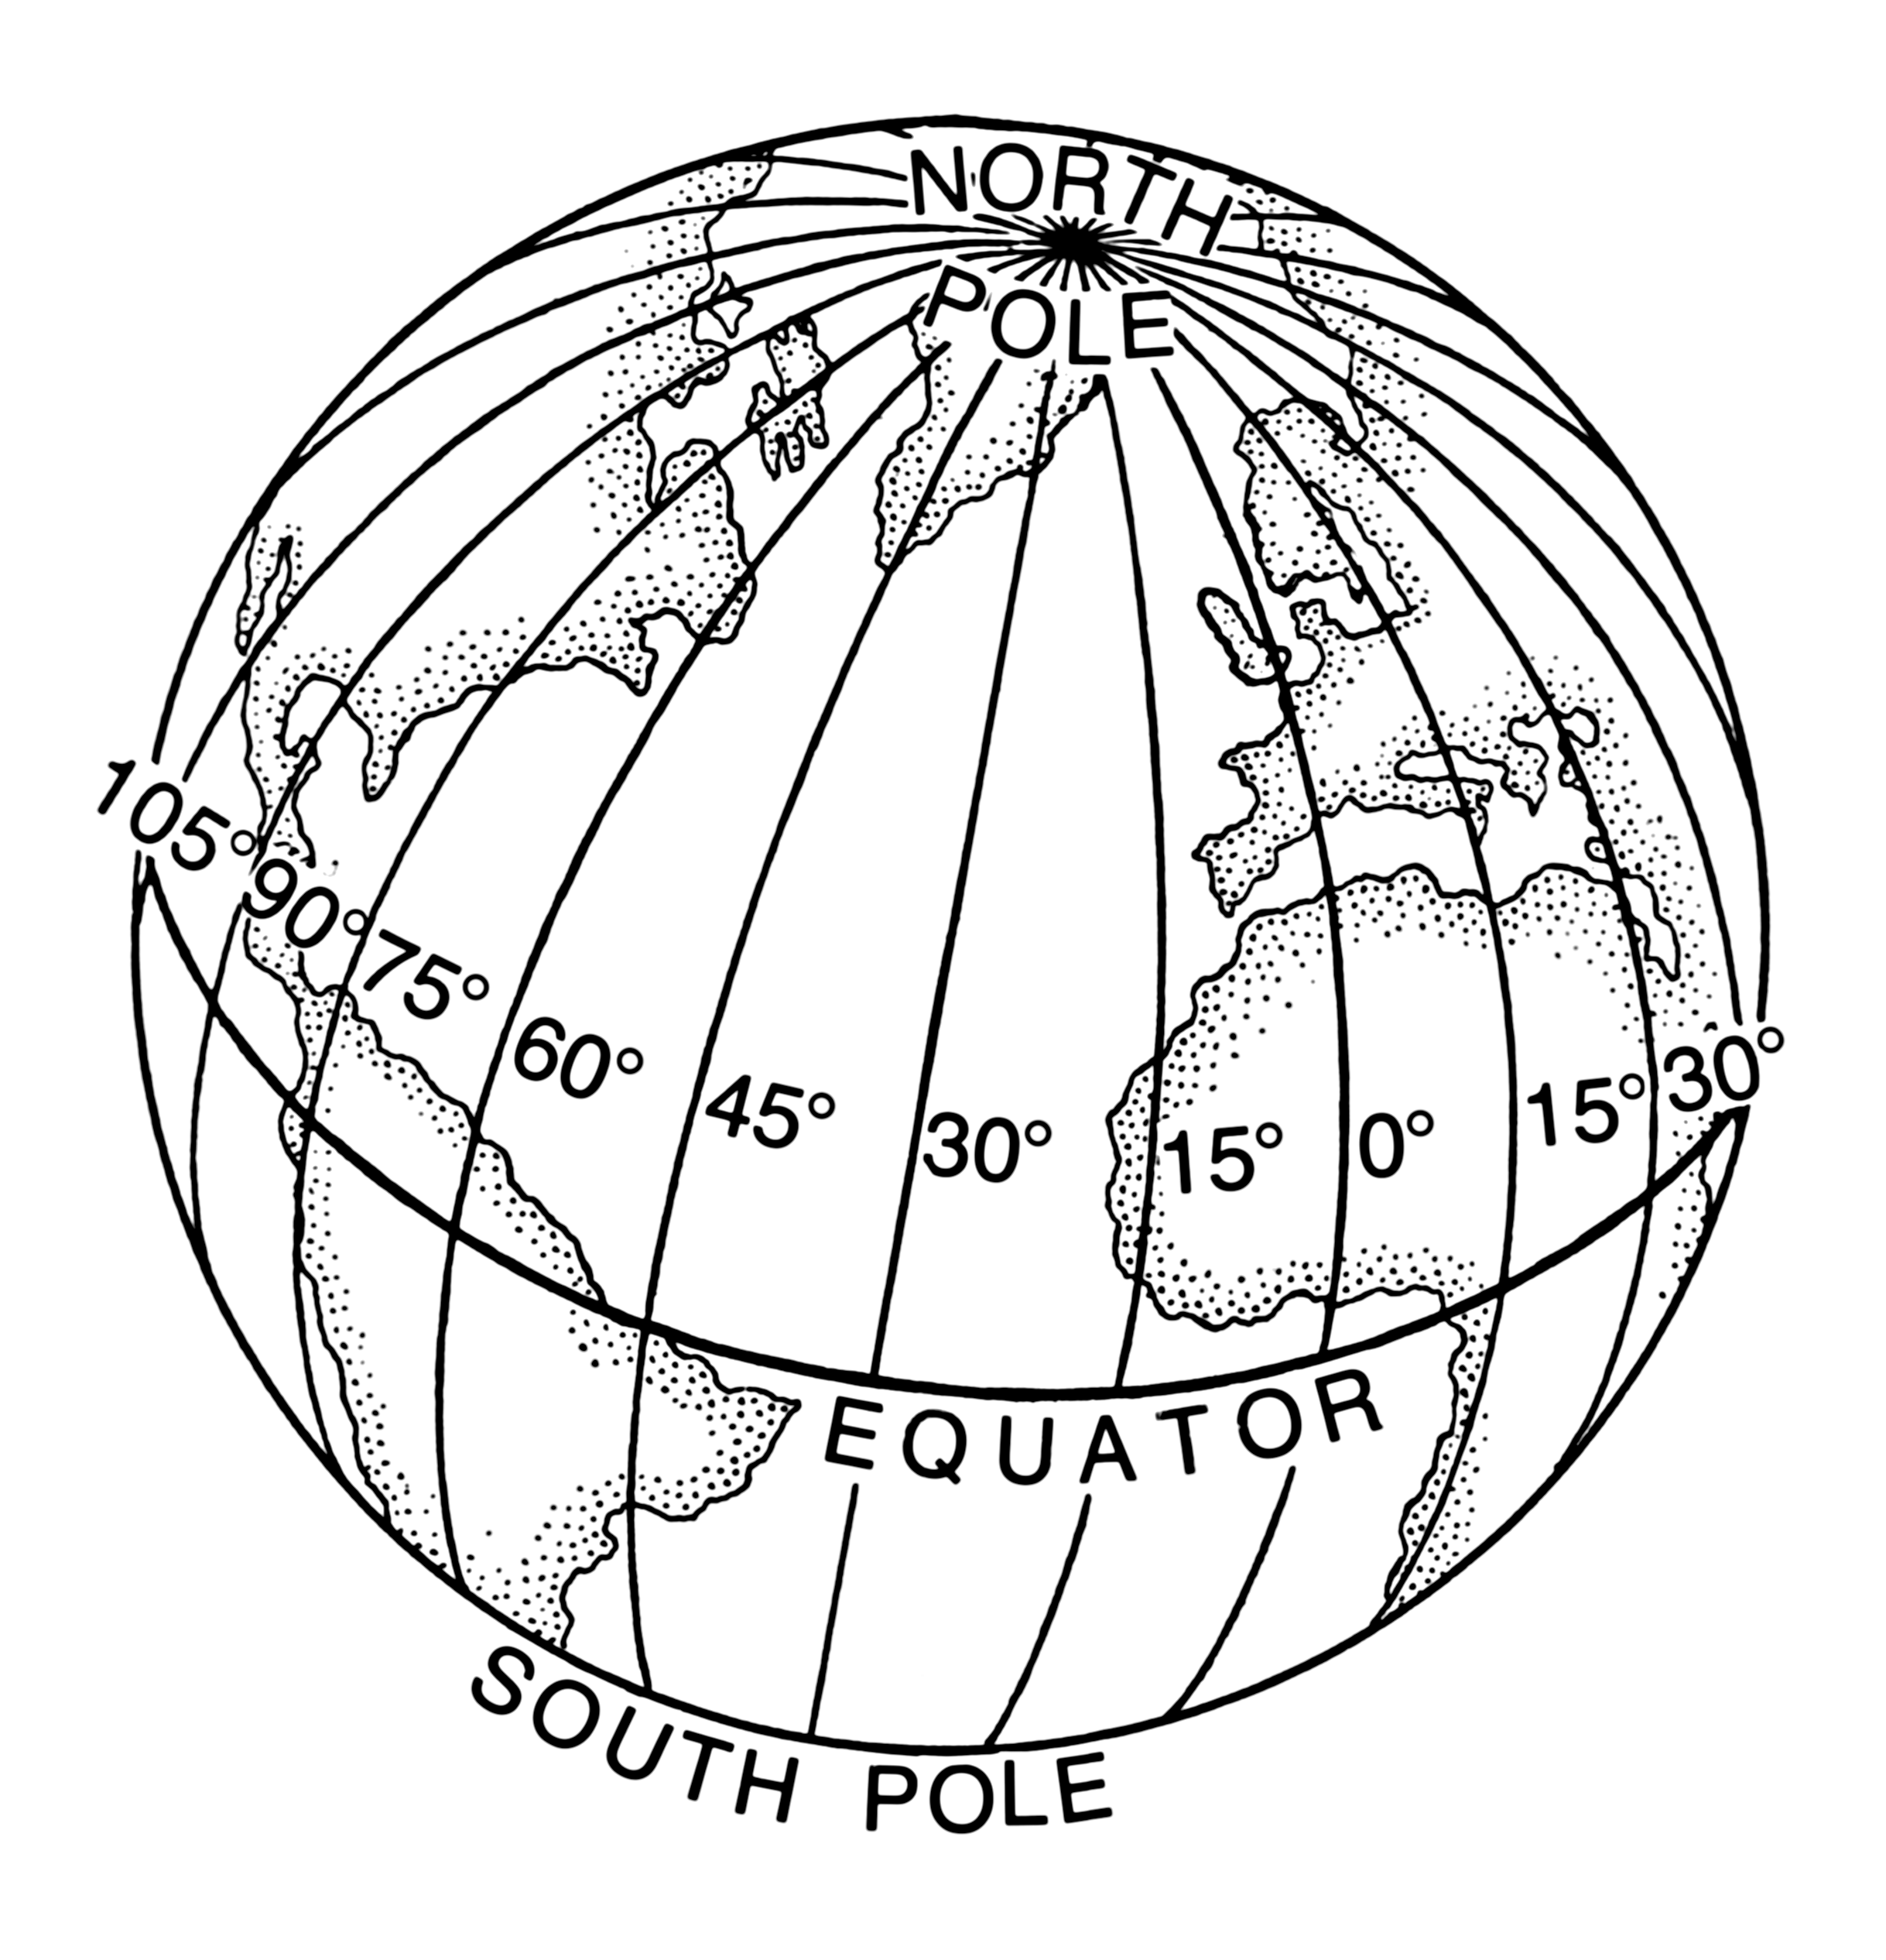
\includegraphics[scale=0.5]{Longitude}\\
Position Nord/Südwest vom Äquator Position west/östlich vom Nullmeridian\\
Sei \lstinline!<p>!ein Prädikat mit Signatur \lstinline!(<t> -> boolean)!.\\
Eine Signatur der Form \lstinline!(predicate <p>! gilt für jeden Wert der Signatur \argt{} sofern (\auf p\zu) \eval \lstinline!#t!\\
Signaturen des Typs \lstinline!predicate <p>)! sind damit \uline{spezifischer} (restriktiver) als die Signatur \argt{} selbst.\\
\lstinline!(define <newt> (signature <t>!\\
\uline{Beispiele:}
\begin{lstlisting}
(define farbe
	(signature (one-of "Blatt" "Herz" "Blatt" "Eichel" "Schell")))
\end{lstlisting}
\pagebreak
\racket{predicate Signaturen am Beispiel von Längen- und Breitengrade}{Restriktive Signaturen mit predicate}{latandlong}
\section{7.5.2015}
Man kann jedes \lstinline!one-of! durch ein \lstinline!predicate! ersetzen.
\lstinputlisting[caption={[Ersetzung one-of druch predicate Siganturen]Das ''gro\ss e One-of Sterben des Jahres 2015''},frame=single]{oneoftopredicate.rkt}
 \ \bigskip\\
Geocoding: Übersetze eine Ortsangabe mittels des Google Maps Geocoding API (Application Programm Interface) in eine Position auf der Erdkugel.\\
\lstinline!(: geocoder (string -> (mixed geocode geocode-error)))!\\
Ein geocode besteht aus: \\
\begin{tabular}{clll}
& \underline{Signatur}\\
- & Adresse & (address) & string\\
- & Ortsangabe & (loc) & location\\
- & Nordostecke & (northeast) & location\\
- & Südwestecke & (southwest) & location\\
- & Typ & (type) & string\\
- & Genauigkeit & (accuracy) & string
\end{tabular}\\
\begin{lstlisting}
(: geocode-adress (geocode -> string))
(: geocode-loc (geocode -> location))
(: geocode-... (geocode -> ...))
\end{lstlisting}
Ein geocode-error besteht aus:\\
\begin{tabular}{clll}
& \underline{Signatur}\\
- & Fehlerart & (level) & (one-of "TCP'' "HTTP'' "JSON'' ''API'')\\
- & Fehlermeldung & (message) & string\\
\end{tabular}\\
\underline{Gemischte Daten}\\
Die Signatur
\begin{lstlisting}
(mixed @\argt{1}@ ... @\argt{n}@)
\end{lstlisting}
ist gültig für jeden Wert, der mindestens eine der Signaturen \argt{1} $\ldots$ \argt{n} erfüllt.\\
\underline{Beispiel:} Data-Definition\\
Eine Antwort des Geocoders ist \underline{entweder}\\
\begin{enumerate}[-]
\i ein Geocode (geocode) \underline{oder}
\i eine Fehlermeldung (geocode-error)
\end{enumerate}
Beispiel (eingebaute Funktion string-\zu number)
\begin{lstlisting}
(: string->number (string -> (mixed number (one-of #f))))
(string->number "42") @\eval@ 42
(string-> number "foo") @\eval@ #f
\end{lstlisting}
\lstinputlisting[literate={ü}{{\"u}}1 {ä}{{\"a}}1,frame=single,caption={[Geocoding] Die Google Geocode API}]{geocoding.rkt}
Erinnerung:\\
Das Prädikat \argt{}? einer Signatur \argt{} unterscheidet Werte der Signatur \argt{} von allen anderen Werten:\\
\lstinline!(: @\argt{}@? (any -> boolean))!\\
Auch: Prädikat für eingebaute Signaturen
\begin{lstlisting}
number?
complex?
real?
rational?
integer?
natural?
string?
boolean?
\end{lstlisting}
Prozeduren, die gemischte Daten der Signaturen \argt{1} $\ldots$ \argt{n} konsumieren: \\
\underline{Konstruktionsanleitung}:\\
\begin{lstlisting}
(: @\argt{}@ ((mixed @\argt{1}@ ... @\argt{n}@) -> ...))
(define @\argt{}@
	(lambda (x)
		(cond 
		   ((@\argt{1}@? x)...)
		   ...
		   ((@\argt{n}@? x) ...))))
\end{lstlisting}
Mittels \underline{let} lassen sich Werte an \underline{lokale Namen} binden,
\begin{lstlisting}
(let ( 
	(@\argid{1}@ @\arge{1}@)
	(...)
	(@\argid{n}@ @\arge{n}@))
 @\arge{}@
) 
\end{lstlisting}
Die Ausdrücke \arge{1} $\ldots$ \arge{n} werden \uline{parallel} ausgewertet. $\Rightarrow$ \argid{1} $\ldots$ \argid{n}  können in \arge{} (und nur hier) verwendet werden. Der Wert des let Ausdruckes ist der Wert von \arge{}.
\racket{cond mit gemischten Daten}{Liegt der Geocode r auf der südlichen Erdhalbkugel?}{hemisphere}
\underline{ACHTUNG:}\\
'let' ist verfügbar auf ab der Sprachebene "Macht der Abstraktion".
\bigskip\\
'let' ist syntaktisches Zucker.
\begin{lstlisting}
(let (			((lambda (@\argid{1}@ ... @\argid{n}@) 
	(@\argid{1}@ @\arge{1}@)		@\arge{}@)
	(...)		@$\equiv$@        @\arge{1}@
	(@\argid{n}@ @\arge{n}@))	       @\arge{2}@ ...
 @\arge{}@			     @\arge{n}@
) 
\end{lstlisting}
\section{12.5.2015}
Abstand zweier geographischer Positionen $b_1,b_2$ auf der Erdkugel in km (lat, lng jeweils in Radian).\\
\begin{mdframed}
\code{Abstand zweier geographischer Positionen l1, l2 auf der\\ 
 Erdkugel in km (lat, lng jeweils in Radian):\\
 \ \\
 dist(l1,l2) =\\
   Erdradius in km *
   acos(cos(l1.lat) * cos(l1.lng) * cos(l2.lat) * cos(l2.lng) + 
        cos(l1.lat) * sin(l1.lng) * cos(l2.lat) * sin(l2.lng) +
        sin(l1.lat) * sin(l2.lat)) }\end{mdframed}
\begin{lstlisting}[frame = single]
; @\latexcode{$\pi$}@
(define pi 3.141592653589793)

; Konvertiere Grad d in Radian (@\latexcode{$\pi$}@ = @\latexcode{$180^{\circ}$}@)
(: radians (real -> real))
(check-within (radians 180) pi 0.001)
(check-within (radians -90) (* -1/2 pi) 0.001)
(define radians
  (lambda (d)
    (* d (/ pi 180))))


; Abstand zweier Orte o1, o2 auf Erdkugel (in km)
; [Wrapper]
(: distance (string string -> real))
(check-within (distance "Tübingen" "Freiburg") (distance "Freiburg" "Tübingen") 0.001)
(define distance
  (lambda (o1 o2)
    (let ((dist (lambda (l1 l2)             ; Abstand zweier Positionen l1, l2 (in km)  [Worker]
                  (let ((earth-radius 6378) ; Erdradius (in km)                  
                        (lat1 (radians (location-lat l1)))
                        (lng1 (radians (location-lng l1)))
                        (lat2 (radians (location-lat l2)))
                        (lng2 (radians (location-lng l2))))
                    (* earth-radius
                       (acos (+ (* (cos lat1) (cos lng1) (cos lat2) (cos lng2))
                                (* (cos lat1) (sin lng1) (cos lat2) (sin lng2))
                                (* (sin lat1) (sin lat2))))))))
          (gc1 (geocoder o1))
          (gc2 (geocoder o2)))
      (if (and (geocode? gc1)
               (geocode? gc2))
          (dist (geocode-loc gc1) (geocode-loc gc2))
          (violation "Unknown location(s)")))))

; ... einmal quer durch die schöne Republik
(distance "Konstanz" "Rostock")
\end{lstlisting}
\underline{\textsc{Parametrisch Polymorphe Prozeduren}}\\
Beobachtung: Manche Prozeduren arbeiten unabhängig von den Signaturen ihrer Argumente : \underline{parametrisch polymorphe Funktion} (griechisch : vielgestaltig).\\
Nutze \underline{Signaturvariablen} \%a , \%b,...\\
Beispiel:\\
\begin{lstlisting}
; die Identität
(: id (%a -> %a))
(define id
  (lambda (x) x))

; die konstante Funktion
(: const (%a %b -> %a))
(define const
  (lambda (x y) x))

; die Projektion
(: proj ((one-of 1 2) %a %b -> (mixed %a %b)))
(define proj
  (lambda (i x y)
    (cond ((= i 1) x)
          ((= i 2) y))))
\end{lstlisting}
Eine polymorphe Signatur steht für alle Signaturen, in denen die Signaturvariablen durch konkrete Signaturen ersetzt werden.\\
Beispiel: Wenn eine Prozedur \code{(: number \%a \%b -\zu \%a)} erfúllt, dann auch:\\
\begin{tabular}{lcl}
\code{(: number string boolean}&\code{ -\zu}& \code{string)} \\
\code{(: number boolean natural}&\code{ -\zu}& \code{boolean)} \\
\code{(: number number number}&\code{ -\zu}& \code{number)} \\
\end{tabular}
\vspace*{1cm}\\
\fbox{''x''}\fbox{23}\hspace*{1cm} \fbox{2}\fbox{\#f}\\
\begin{lstlisting}
; Ein polymorphes Paar (pair-of %a %b) besteht aus
; - einer ersten Komponente (first)
; - einer zweiten Komponente (rest)
(: make-pair (%a %b -> (pair-of %a %b)))
(: pair? (any -> boolean))
(: first ((pair-of %a %b) -> %a))
(: rest  ((pair-of %a %b) -> %b))
(define-record-procedures-parametric pair pair-of
  make-pair
  pair?
  (first
   rest))
\end{lstlisting}
\code{(pair-of \argt{1} \argt{2})} ist eine Signatur für Paare deren erster bzw. zweiter Komponente die Signaturen \argt{1} bzw. \argt{2} erfüllen.\\
\begin{lstlisting}
;@\latexcode{$\rightarrow$}@ pair-of Signatur mit (zwei) Parametern
(: make-pair (\%a \%b -> (pair-of \% a \%b)))
(: pair? (any -> boolean))
(: first ((pair-of %a %b ) -> %a))
(: rest ((pair-of %a %b ) -> %b))
\end{lstlisting}
\begin{lstlisting}[frame=single]
; Ein paar aus natürlichen Zahlen
; FIFA WM 2014
(: deutschland-vs-brasilien (pair-of natural natural))
(define deutschland-vs-brasilien
  (make-pair 7 1)) 

; Ein Paar aus einer reellen Zahl (Messwert) 
; und einer Zeichenkette (Einheit)
(: measurement (pair-of real string))
(define measurement
  (make-pair 36.9 "@$^{\textcolor{string}{\circ}}$@C"))


; "Liste" der Zahlen 1,2,3,4
(define nested
  (make-pair 1
             (make-pair 2
                        (make-pair 3
                                   4))))

; Extrahiere das dritte Element der Liste (hier: 3)
(first (rest (rest nested)))
\end{lstlisting}
Eine \underline{Liste} von Werten der Signatur \argt{t} ist entweder\\
\begin{enumerate}[-]
\i leer (Signatur \code{empty-list}) oder:\\
\i ein Paar (Signatur \code{pair-of}) aus einem Wert der Signatur \argt{} und einer Liste von Werten der Signatur \argt{}. \\
\end{enumerate}
\begin{lstlisting}
(define list-of
  (lambda (t)
    (signature (mixed empty-list
                      (pair-of t (list-of t))))))

\end{lstlisting}
Signatur \code{empty-list} bereits in Racket vordefiniert.\\
Ebenfalls vordefiniert:\\
\code{(:empty empty-list)}\\
\code{(: empty? (any -\zu boolean))}\\
\underline{Operatoren auf Listen}\\
\begin{enumerate}
\i[Konstruktoren]
\begin{tabular}{ll}
\code{(: empty-list)}& leere liste\\
\code{(: make-pair (\% a (list-of \% a))} & Konstruire Liste aus Kopf und Rest
\end{tabular}
\i[Predikate:]
\begin{tabular}{ll}
\code{(: empty (any -\zu boolean)}& liegt leere Liste vor?\\
\code{(: pair? (any -\zu boolean))} & Nicht leere Liste?
\end{tabular}
\i[Selektoren:]
\begin{tabular}{ll}
\code{(: first (list-of \%a) -\zu \%a)}& Kopf-Element\\
\code{(: rest (list-of \%a) -\zu (list-of \%a))} & Rest Liste
\end{tabular}
\end{enumerate}
\begin{lstlisting}[frame=single]
; Noch einmal (jetzt mit Signatur): Liste der natürlichen Zahlen 1,2,3,4
(: one-to-four (list-of natural))
(define one-to-four
  (make-pair 1
             (make-pair 2
                        (make-pair 3
                                   (make-pair 4
                                              empty)))))


; Eine Liste, deren Elemente natürliche Zahlen oder Strings sind
(: abstiegskampf (list-of (mixed number string)))
(define abstiegskampf
  (make-pair "SCF"
             (make-pair 96
                        (make-pair "SCP"
                                   (make-pair "VfB" empty)))))

\end{lstlisting}
\section{19.5.2015}
\code{(make-pair 1 (make-pair 2 empty))}\\
\uline{Visualisierung Listen}\\ \ \\
\begin{tikzpicture}
\draw[black,solid] (0,0)--(0,1);
\draw[black,solid] (0,0)--(4.5,0);
\draw[black,solid] (0,1)--(4.5,1);
\draw[black,solid] (4.5,1)--(4.5,0);
\draw[black,solid] (1.5,1)--(1.5,0);
\node () at (0.75,0.5) {1};
\draw[black,solid] (1.75,0.25)--(4.25,0.25);
\draw[black,solid] (1.75,0.75)--(4.25,0.75);
\draw[black,solid] (1.75,0.75)--(1.75,0.25);
\draw[black,solid] (4.25,0.75)--(4.25,0.25);
\node () at (2.25,0.5) {2};
\draw[black,solid] (3.0,0.75)--(3.0,0.25);\\
\node () at (3.62,0.5) {empty};
\end{tikzpicture}\\ \ \\
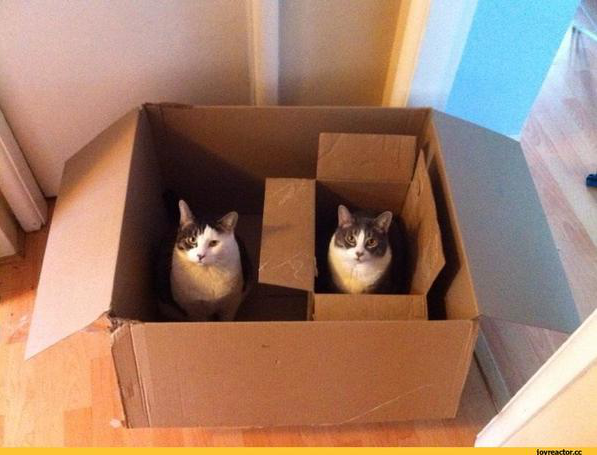
\includegraphics{katzenbabies}
\uline{Spine (Rückgrat)}\\
\code{(pair-of natural (list-of natural))}\\
\begin{tikzpicture}
\node () at (-1.5,0.5) {\code{(natural first)}};
\node () at (3.25,0.5) {\code{ rest (list-of natural)}};
\draw[black,solid] (0,0)--(0,1);
\draw[black,solid] (0,0)--(1,0);
\draw[black,solid] (0,1)--(1,1);
\draw[black,solid] (1,1)--(1,0);
\draw[black,solid] (0.5,1)--(0.5,0);
\node () at (0.25,0.5) {1};
\draw[black,solid] (0.75,0.5)--(1.5,-0.75);
\draw[black,solid] (1.5,-0.75)--(1.5,-1.75);
\draw[black,solid] (1.5,-0.75)--(2.5,-0.75);
\draw[black,solid] (1.5,-1.75)--(2.5,-1.75);
\draw[black,solid] (2.5,-1.75)--(2.5,-0.75);
\draw[black,solid] (2.0,-1.75)--(2.0,-0.75);
\node () at (1.75,-1.25) {2};
\draw[black,solid] (2.25,-1.25)--(3,-2.5);
\node () at (3,-2.75) {\code{empty}};
\end{tikzpicture}\\
\begin{lstlisting}[frame=single]
(: one-to-four (list-of natural))
(define one-to-four
  (make-pair 1 
             (make-pair 2 
                        (make-pair 3 
                                   (make-pair 4 
                                              empty)))))  
\end{lstlisting}
\code{(: jedis-and-siths (list-of (list-of string)))}\bigskip\\ 
\begin{tikzpicture}
\node () at (0,5) {};
\draw (6,6) rectangle (5,5);
\draw[black,solid] (5.5,6)--(5.5,5);
\draw[black,solid] (5.25,5.5)--(4.5,4.5);
\draw[black,solid] (5.75,5.5)--(8.5,4.5);
\draw (8.5,4.5) rectangle (9.5,3.5);
\draw[black,solid] (9.25,4)--(9.8,3.3);
\node () at (9.8,3.1) {\code{empty}};

\draw[black,solid] (8.75,4)--(7.5,3);
\draw (7.5,3) rectangle (8.5,2);
\draw (8,3)--(8,2);
\draw (7.75,2.5)--(7,2);
\node () at (7,1.75) {\textcolor{string}{''Doku''}};

\draw (8.25,2.5)--(9,2);
\draw[black,solid] (9,2) rectangle (10,1);
\draw (9.5,2)--(9.5,1);
\draw (9.75,1.5)--(10.5,0.5);
\node () at (10.5,.25) {\code{empty}};
\draw (9.25,1.5)--(8.75,0.5);
\node () at (8.75,0.25) {\textcolor{string}{''Darth''}};


\draw[black,solid] (9,3.5)--(9,4.5);
\draw (4.5,4.5) rectangle (3.5,3.5);
\draw[black,solid] (4,4.5)--(4,3.5);
\draw (3.75,4)--(3.3,3.3);
\node () at (3.2,3.1) {\textcolor{string}{''Obi''}};
\draw (4.25,4)--(5,2.5);
\draw (5,2.5) rectangle (6,1.5);
\draw (5.5,2.5)--(5.5,1.5);
\draw (5.25,2)--(4.5,1);
\draw (5.75,2)--(6.5,1);
\node () at (4.5,0.8) {\textcolor{string}{''Yoda''}};
\node () at (6.5,0.8) {\code{empty}};
\end{tikzpicture}
\begin{lstlisting}[frame=single]
; Geschachtelte Listen
(: jedis-and-siths (list-of (list-of string)))
(define jedis-and-siths
  (MAKE-PAIR (make-pair "Yoda"
                        (make-pair "Obi-Wan" empty))
             (MAKE-PAIR (make-pair "Dooku"
                                   (make-pair "Vader" empty))
                        empty)))

; Navigation in geschachtelten Listen
(check-expect (first (first jedis-and-siths)) "Yoda")
(check-expect (first (rest (first (rest jedis-and-siths)))) "Vader")
\end{lstlisting}
\uline{Prozeduren, die Liste konsumieren}\\
Konstruktionsanleitung:\\
Beispiel:\\
\begin{lstlisting}
(: list-sum ((list-of number) -> number))

(check-expect (list-sum empty) 0)
(check-expect (list-sum (make-pair 40
                                   (make-pair 2
                                              empty))) 42)  
(check-expect (list-sum one-to-four) 10)

(define list-sum
  (lambda (xs)
    (cond ((empty? xs) 0)
          ((pair? xs) (+ (first xs)
                         (@{\uline{list-sum} (rest xs)))))))
\end{lstlisting}
\begin{figure}[htbp]
\begin{minipage}[b]{\textwidth}
\begin{tikzpicture}
\node () at (0,0) {};
\draw (2,2) rectangle (3,2.5);
\node () at (1.55,2.25) {xs:};
\draw (2.5,2.5)--(2.5,2);
\draw (2.25,2.25)--(1.5,1.5);
\node () at (1.5,1.25) {x};
\draw (2.75,2.25)--(5.5,0.5);
\draw (3.5,1.75)--(2,0.5);
\draw (2,0.5)--(5.5,0.5);
\node () at (3.75,0.8) {\code{(rest xs)}};
\end{tikzpicture}
\hspace*{2cm}
\begin{minipage}[b]{0.3\textwidth}
\code{(rest xs)} mit Signatur \code{(list-of number)} ist selbst wieder eine \uline{kürzere} \uline{Liste} von Zahlen.\\
\code{(list sum (rest xs))} erzielt Fortschritt
\end{minipage}
\end{minipage}
\end{figure}
Konstruktionsanleitung für Prozeduren:
\begin{lstlisting}
(: <f> ((list-of @\argt{1}@) -> @\argt{2}@))
(define <f>
	(lambda(xs)
		(cond 
			((empty? xs) ...)
			((pair? xs) ... @$\overbrace{\text{(first xs)}}^{\text{\argt{1}}}$@ ...)
				(<f> @$\underbrace{\text{(rest xs )}}_{\text{\argt{1}}}$@))...))
\end{lstlisting}
Neue Sprachebene ''Macht der Abstraktion''
\begin{enumerate}[-]
\i Signatur \code{(list-of \% a)} eingebaut
\begin{lstlisting}
(list @\arge{1}@ @\arge{2}@ ... @\arge{n}@)
	@$\equiv$@
(make-pair (@\arge{1}@)
	(make-pair @\arge{2}@)
		... (make-pair @\arge{n}@) empty) ...)
\end{lstlisting}
\i Ausgabeformat für nicht leere Listen:\\
\code{\#\auf list $x_1 \ x_2 \ \ldots \ x_n$\zu}
\end{enumerate}
\begin{lstlisting}[frame=single]
; Länge der Liste xs
(: list-length ((list-of %a) -> natural))

(check-expect (list-length empty) 0)
(check-expect (list-length (list 1 1 3 8)) 4)
(check-expect (list-length jedis-and-siths) 2)    ; nicht 4!

(define list-length
  (lambda (xs)
    (cond ((empty? xs) 0)
          ((pair? xs) (+ 1 
                         (list-length (rest xs)))))))
  
\end{lstlisting}
Füge Listen xs , ys zusammen (con\uline{cat}ination)\\
Zwei Fälle (xs leer oder nicht leer)
\begin{enumerate}
\i[\circled{1}] $\overbrace{ \text{\code{empty}}}^{\text{xs}} \ \ \overbrace{y_1 \ y_2 \ \ldots \ y_m}^{ys}
 \ \ \overbrace{y_1 \ y_2 \ \ldots \ y_m}^{\text{\code{(cat \ xs \ ys)}}}$
\i[\circled{2}] $x_1 \ \underbrace{x_2 \ \ldots \ x_n}_{\text{\code{(rest xs)}}} \ y_1 \ y_2 \ \ldots \ y_m \ \ x_1 \ \underbrace{ x_2 \ldots \ x_n \ y_1 \ y_2 \ \ldots \ y_m}_{\text{\code{(cat rest xs)}}}$
\end{enumerate}

Beobachtung:
\begin{enumerate}[-]
\i Die Längen von xs bestimmt die Anzahl der rekursiven Aufrufe von cat
\i Auf xs werden \uline{Selektoren angewendet}
\end{enumerate}
\begin{lstlisting}[frame=single]
; Füge Listen xs, ys (in dieser Reihenfolge) zusammen
(: cat ((list-of %a) (list-of %a) -> (list-of %a)))

(check-expect (cat (list 1 2) (list 3 4)) (list 1 2 3 4))
(check-expect (cat one-to-four empty) one-to-four)
(check-expect (cat empty one-to-four) one-to-four)

(define cat
  (lambda (xs ys)
    (cond ((empty? xs) 
           ys)
            ((pair? xs)
             (make-pair (first xs) ; <- cat dennoch param. polymorph
                        (cat (rest xs) ys))))))

; Hinweis: Verfügbar als eingebaute Funktion `append'
\end{lstlisting}
\section{21.5.2015}
\lstinputlisting[frame=single,caption={[Bildmanipulation mit Listen aus Pixeln]Ausflug: Bluescreen Berechnung wie in Starwars mit Listen:}]{bluescreen.rkt}
Generierung aller natürlichen Zahlen (vgl. gemischte Daten)\\
Eine natürliche Zahl (natural) ist entweder 
\begin{enumerate}[-]
\i die 0 (zero)
\i der Nachfolge (succ) einer natürlichen Zahl
\end{enumerate}

$\mathbb{N} = \{0, (succ(0)), (succ(succ(0))), \ldots \} $\\
\uline{Konstruktoren}\\
\begin{lstlisting}
(: zero natural)
(define zero 0)
(: succ (natural -> natural))
(define succ (lambda (n)(+ n 1)))
\end{lstlisting}
Vorgänger (pred), definiert für $n > 0$
\begin{lstlisting}
(: pred (natural -> natural))
(define pred
	(lambda (n) (- n 1)))
\end{lstlisting}
Bedingte algebraische Eigenschaft (für check-property):\\
\lstinline!(==> <p> <t>)!\\
Nur wenn \auf p \zu \eval \# t ist, wird Ausdruck \argt{} ausgwertet und getestet \argt{} \eval \# t
\racket{Check-property mit Einschränkungen}{$==>$ als Einschränkungsoperator}{notquiteall}
Beispiel für Rekursion auf natürlichen Zahlen: Fakultät\\$
\begin{array}{rcl}
0! &=& 1\\
n! &=& n \cdot (n -1)!\\
&\\
3! &=& 3 \cdot 2!\\
&=& 3 \cdot 2 \cdot 1!\\
&=& 3 \cdot 2 \cdot 1 \cdot 0!\\
&=& 3 \cdot 2 \cdot 1 \cdot 1\\
&=& 6\\
&\\
10 &=& 3628800
\end{array}$\bigskip \\
\racket{Rekursion auf natürlichen Zahlen: Fakultät}{Fakultät rekursiv}{Fakultaet}
Konstruktionsanleitung für Prozeduren über natürlichen Zahlen:\\
\begin{lstlisting}
(:<f> (natural -> <t>))
	(define <f>
		(lambda (n)
			(cond ((= n 0)...)
				((> n 0) ... (<f> (- n 1))...))))
\end{lstlisting}
Beobachtung:\\
\begin{enumerate}[-]
\i Im letzten Zweig ist $n > 0 \rightarrow$ pred angewandt
\i \lstinline!(<f> (- n 1))! hat die Signatur \argt{}
\end{enumerate}
Satz:\\
Eine Prozedur, die nach der Konstruktionsanleitung für Listen oder natürliche Zahlen konstruiert wurde \uline{terminiert immer} (= liefert immer ein Ergebnis).\\
(Beweis in Kürze)\\
\racket{Fehlerhafte Rekursionen}{Fehlerhafte Rekursionen}{FehlerRekursiv}
$\overbrace{(3 \cdot (2 \cdot (1}^{\t{merken}} \cdot 0!)))$\\
Die Grö\ss e eines Ausdrucks ist proportional zum Platzverbrauch des Reduktionsprozesses im Rechner\\
$\Rightarrow$ Wenn möglich Reduktionsprozesse, die \uline{konstanten} Platzverbrauch - unabhängig von Eingabeparametern - benötigen
\section{9.6.2015}
Beobachtung: \lstinline!(factorial 10).!\\
\lstinline!(* 10 (* 9 (* 8 (* 7 (* 6(factorial 5))))))!\\
$\underset{\substack{\t{Assozivität}\\
\t{von } \cdot}}{=}$ \lstinline|(*(*(*(*(* 10 9)8)7)6)(factorial 5))| \eval \lstinline|(* 30240 (factorial 5))|\\
$\rightarrow$ Multiplikationen können vorgezogen werden \begin{turn}{}
:-)
\end{turn}\\
Idee: Führe Multiplikation sofort aus. Schleife des Zwischenergebnis ({\em akkumulierendes Argument}) durch die ganze Berechnung. Am Ende erhält der Akkumulatoren das Endergebnis.\\
Beispiel: Berechne 5!\\
\lstinline!(: fac-worker (natural natural -> natural))!\\
\begin{tabular}{l|ll}
n & acc\\
\hline {\tiny-1}\begin{turn}{45}
$\curvearrowleft$
\end{turn}5 & 1 \begin{turn}{-45}
$\curvearrowright$
\end{turn} $\cdot$ {\tiny 5} & neutrales Element\\
{\tiny-1}\begin{turn}{45}
$\curvearrowleft$
\end{turn}4 & 5 \begin{turn}{-45}
$\curvearrowright$
\end{turn} $\cdot$ {4} \\
{\tiny-1}\begin{turn}{45}
{$\curvearrowleft$}
\end{turn}3 & 20 \begin{turn}{-45}
$\curvearrowright$
\end{turn} $\cdot$ {3}\\
{\tiny-1}\begin{turn}{45}
$\curvearrowleft$
\end{turn}2 & 60 \begin{turn}{-45}
$\curvearrowright$
\end{turn} $\cdot$ { 2}\\
{\tiny-1}\begin{turn}{45}
$\curvearrowleft$
\end{turn}1 & 120 \begin{turn}{-45}
$\curvearrowright$
\end{turn} $\cdot$ {1}\\
{\tiny-1}\begin{turn}{45}
$\curvearrowleft$
\end{turn}0 & 120
\end{tabular}
\lstinputlisting[firstline=43, lastline=58]{Endrekursion.rkt}
Ein Berechnungsprozess ist \emph{iterativ}, falls seine Grö\ss e konstant bleibt.\\
Damit:
\par \lstinline|factorial| nicht iterativ
\par \lstinline|fac-worker| iterativ\\
Wieso ist \lstinline|fac-worker| iterativ?\\
Der Rekursive Aufruf ersetzt den aktuell reduzierten Aufruf \emph{vollständig}. Es gibt keinen {\em Kontext} (umgebenden Ausdruck), der auf das Ergebnis des rekursiven Aufrufs ''wartet''\\
Kontext des rekursiven Aufrufs in:\\
\begin{enumerate}[-]
\i \lstinline|factorial|: \hfill \lstinline[mathescape]|(* n $\Box$)|
\i \lstinline|fac-worker|: \hfill keiner
\end{enumerate}
Eine Prozedur ist \emph{endrekursiv} (tail call), wenn sie keinen Kontext besitzt. Prozeduren, die nur endrekursive Prozeduren beinhalten, hei\ss en selber endrekursiv.
Endrekursive Prozeduren generieren {\em iterative} Berechnungsprozesse\\
\lstinline|(: rev ((list-of %a)) -> (list-of %a))|\\
\lstinputlisting[frame=single,firstline=68,lastline=78,caption={[Umdrehen einer Liste durch lambda Rekursion] Liste xs umdrehen}]{Endrekursion.rkt}
Beobachtung: von \lstinline|(rev (from-to 1 1000))|\\
$\overbrace{\t{\lstinline[mathescape]|(cat $\underbrace{\t{(list 1000 ... 2)}}_{\t{(cat (list 1000 ... 3) (list 2))}}$ (list 1))|}}^{\t{1000 $\cdot$ \lstinline!make-pair!}}\\
\rightarrow$ Aufrufe von \lstinline|make-pair|: 1000+999+998+\ldots+1\\
$\sum\limits_{i=1}^{n} i = \frac{n \cdot (n + 1)}{2}$ {\em Quadratische Aufrufe } \begin{turn}{}
:-(
\end{turn}\\
Konstruiere iterative Listenumkehrfunktion \lstinline|backwards|:\\
\lstinline|(: backwards-worker ((list-of %a) (list-of %a) -> (list-of %a)))|
\begin{tabular}{l|l}
n & acc\\
\hline{\tiny \lstinline|rest|}\begin{turn}{45}
$\curvearrowleft$
\end{turn}\lstinline!(list 1 2 3)! & \lstinline[]!(list)! \begin{turn}{-45}
$\curvearrowright$
\end{turn}{\tiny \lstinline|make-pair|}\\
{\tiny \lstinline|rest|}\begin{turn}{45}
{$\curvearrowleft$}
\end{turn}\lstinline!(list 2 3)! & \lstinline[]!(list 1)! \begin{turn}{-45}
$\curvearrowright$
\end{turn}{\tiny \lstinline|make-pair|}\\
{\tiny \lstinline|rest|}\begin{turn}{45}
$\curvearrowleft$
\end{turn}\lstinline!(list 3)! & \lstinline[]!(list 2 1)! \begin{turn}{-45}
$\curvearrowright$
\end{turn}{\tiny \lstinline|make-pair|}\\
\lstinline!empty!& \lstinline!(list 3 2 1)!\\
\end{tabular}\bigskip\\
Mittels \lstinline!letrec! lassen sich Werte an lokale Namen binden.
\begin{lstlisting}
(letrec 
	((@\argid{1}@ @\arge{1}@) ...
	(@\argid{n}@ @\arge{n}@))@\arge{}@)
\end{lstlisting}
Die Ausdrücke \arge{1},\ldots,\arge{n} und \arge{} dürfen sich auf die Namen \argid{1}\ldots \argid{n} beziehen
\lstinputlisting[firstline=82,lastline=100,frame=single,caption={[Letrec und endrekursives Umdrehen einer Liste]Effizientere Variante eine Liste umzudrehen}]{Endrekursion.rkt}

\section{11.6.2015}
\emph{Induktive Definition}\\
Konstante Definition der natürlichen Zahlen $\mathbb{N}$.\\
Definition: (Peamo Axiome)
\begin{align}
	0 \in& \mathbb{N} \tag{P1} \\
	\forall n \in& \mathbb{N}: succ(n) \in \mathbb{N} \tag{P2}\\
	\forall n \in& \mathbb{N}: succ(n) \ne 0 \tag{P3}\\
	\forall n,m \in& \mathbb{N} : succ(n) = succ(m) \Leftrightarrow n = m \tag{P4}
\end{align}\\
TODO: "Plot" mit punkten und Pfeilen
\begin{multline}
	\t{Für jede Menge }M \subset N \t{ mit } 0 \in M \\
	\t{und } \forall n : (n \in M \Rightarrow succ(n) \in M), \t{gilt } M = \mathbb{N} \tag{P5}
\end{multline}
''$\mathbb{N}$ enthält nicht mehr als die 0 und die durch $succ()$ generierten Elemente\\
''Nicht ist sonst in $\mathbb{N}$,\\
TODO: Plot von zwei kreisen ineinander
Beweisschema der {\em vollständigen Induktion}\\
Sei $P(n)$ eine Eigenschaft einer Zahl $n \in \mathbb{N}$\\
\lstinline|(: P (natural -> boolean))|\\
Ziel : $\forall n \in \mathbb{N} : P(n)$\\
Definiere $M = \{n \in \mathbb{N} \vert P(n) \} \subset \mathbb{N}$\hfill
M enthält die Zahlen n für die $P(n)$ gilt \\
\emph{Induktionsaxiom}\\
Falls \par 0 $\in M$\\
und \par $\forall n : (n \in M \Rightarrow succ(n) \in M)$\\
dann \par $M \in \mathbb{N}$\\
\begin{minipage}[c]{0.235\textwidth}
	Induktionsstart\bigskip\\
	\ \\
	Induktionsschritt
\end{minipage}
\begin{minipage}[c]{0.765\textwidth}
	\begin{mdframed}
		Falls \par $P(0)$\\
		und \par $\forall (P(n) \Rightarrow P(succ(n))$\\
		dann \par $\forall n \in \mathbb{N} P(n)$
	\end{mdframed}
\end{minipage}
{\em Beispiel}:\\
$\begin{array}{ll}
1 & = 1\\
1 + 3 & = 4\\
1 + 3 + 5 & = 9\\
1 + 3 + 5 + 7 & = 16\\
\ldots\\
P(n) & = \underbrace{\sum\limits_{i=0}^{n} (2i + 1)}_{\substack{\t{Summe der}\\
			\t{ersten n}\\
			\t{ungeraden Zahlen}}} \overset{!}{=} (n+1)^2
\end{array}$\\
\emph{Induktionsschluss P(0)}\\
$\sum\limits_{0}^{0} (2i + 1) = 2 \cdot 0 + 1 = (0 + 1)^ 2 \checkmark$\\
Induktionsschritt $\forall n (P(n)) = P (n+1)\\
\begin{array}{ll}
\sum\limits_{i=0}^{n+1} (2i + 1) &\overset{\sum}{=} \sum\limits_{i=0}^{n} (2i + 1) + (2 (n+1) +1)\\
&\overset{iv.}{=} (n+1)^2 + 2n +3\\
&= n^2 + 4n + 4\\
 &= ((n+1)+1)^2 \checkmark
\end{array}$\\
{\em Beispiel}:\\
\begin{lstlisting}
	(define factorial 
		(lambda (k)
			(if 
				(= k 0) 1
				(* k (factorial (- k 1))))))
\end{lstlisting}
$P(x) \equiv \text{\lstinline!(factorial n)!} = \fbox{n!}$ \hfill $\fbox{x}$:(Racket Repräsentation für $x \in \mathbb{N}$)\\
Zeige : $\forall n \in \mathbb{N} : P(n)$\\
\emph{Induktionsbasis $P(0)$}\\
\lstinline[mathescape]!(factorial($\numrak{0}$))!\\
\begin{enumerate}[\eval]
\i[$\overset{\star}{\text{\eval}}$] \lstinline[mathescape]!((lambda (k)...)$\numrak{0}$)!
\i \lstinline[mathescape]|(if (= $\numrak{0}$ 0)1 ...)|
\i \lstinline[]|(if #t|\lstinline| 1 ...)|
\i 1 = \numrak{0}! $\checkmark $
\end{enumerate}
Induktionsschritt: $\forall n : (P(n) \rightarrow P(n+1))$\\
\lstinline[mathescape]|(factorial $\numrak{n+1}$)|
\begin{enumerate}[\eval]
\i[$\overset{\star}{\text{\eval}}$] \lstinline[mathescape]|((lambda (n)...)$\numrak{n+1}$)|\\
\i \lstinline[mathescape]|(if (= $\numrak{n+1}$ 0)1 ... (...))|
\i \lstinline[]|(if #f|\lstinline| 1 ... (...))|
\i \ \marginpar{\flushleft \textcolor{red}{Unter der Annahme, dass tatsächlich Subtraktion implementiert ist}} \lstinline[mathescape]|(* $\numrak{n+1}$ (factorial (- $\numrak{n+1}$ 1)))|
\i \lstinline[mathescape]|(* $\numrak{n+1}$ (factorial $\numrak{n}$))|
\i[$\overset{iv}{=}$] \lstinline[mathescape]|(* $\numrak{n + 1}$ n!)|
\i[=]$(n+1)!\ \checkmark$
\end{enumerate}
\emph{Beispiel}:\\
Jede durch die Konstruktionsanleitung für Funktionen über natürliche Zahlen konstruierte Funktion liefert ein Ergebnis ({\em terminiert immer})\\
\begin{lstlisting}
(define f
	(lambda (n)
		(if
			(= n 0) base
			(step (f (n-1)) n))))
\end{lstlisting}
\lstinline|(: base natural)|\\
\lstinline|(: step (natural natural -> natural))|
Bsp: step $\rightarrow$ \lstinline|(lambda (x y) (* x y))|\\
Dann gilt $P(n)$ = \lstinline!(f n)! terminiert (Mit Ergebnis der Signatur \lstinline!natural!)\\
Zeige $\forall n \in \mathbb{N} : P(n)$\\
\emph{Induktionsbasis P(0)}:\\
\lstinline[mathescape]|(f $\numrak{0}$)|
\begin{enumerate}[\eval]
\i \lstinline[mathescape]|(if (= $\numrak{0}$ 0) base ...)|
\i \lstinline[]|(if #t base|
\i base $\checkmark $
\end{enumerate}
Induktionsschritt $\forall n : (P(n) \rightarrow P(n+1))$\\
\lstinline[mathescape]|(f $\numrak{n+1}$)|
\begin{enumerate}[\eval]
	\i \lstinline[mathescape]|(if (= $\numrak{n+1}$ 0) base ... (step ...))|
	\i \lstinline[]|(if #f|\lstinline| base ... (step ...))|
	\i \lstinline[mathescape]|(step (f (- $\numrak{n+1}$ 1)) $\numrak{n+1}$)|
	\i \lstinline[mathescape]|(step $\underbrace{(f \numrak{n})}_{\t{terminiert}}$ $\numrak{n+1}$)|
	\i[$\Rightarrow$]\lstinline[mathescape]!(step (f $\numrak{n}$) $\numrak{n+1}$)! terminiert
\end{enumerate}
\emph{Definition}:(Listen.endliche Folge)\\
Die Menge $M^*$ (= Listen mit Elementen aus $M$ + \lstinline|list-of M| ist \emph{induktiv} definiert\\
\begin{align}
\text{\lstinline!empty!} \in& M^* \tag{L1} \marginnote{Nicht leere Liste}\\
\forall x \in& M , xs \in M^* \tag{L2} \marginnote{\flushright \text{\lstinline!(make-pair x xs)!}}\marginnote{\t{$\in M^*$}} \\
\t{Nichts sonst in }& M^* \tag{L3}
\end{align}
Beweisschema \emph{Listeninduktion}\\
So $P(xs)$ eine Eigenschaft von Listen über M.\\
\lstinline|(: P ((list-of M) -> boolean))|\\
\begin{mdframed}
	Falls $P(\text{\lstinline|empty|})$ \marginnote{Induktionsanfang}\\
	und \par$\forall x \in M, xs : P(xs) \Rightarrow (P(xs) \Rightarrow (P($\lstinline|make-pair x xs|))\\
	dann \par $\forall xs \in M^* : P(xs)$ \marginnote{Indukstionsschritt}
\end{mdframed}
\newpage
\section{16.6.2015}
\emph{Beispiel}:\\
\begin{lstlisting}
(define cat
	(lambda (xs ys)
		(cond
			((empty? xs ) ys)
			((pair? xs) (make-oair (first xs) (cat (rest xs) ys))))))
\end{lstlisting}

$\begin{cases}
	(1) & \text{\lstinline|cat empty ys| = ys}\\
	\marginnote{($M^*$, \lstinline|cat|,\lstinline|empty| ist ein \emph{Monoid})}(2) & \text{\lstinline|(cat xs empty)| = xs}\\
	(3) & \text{\lstinline|(cat (cat xs ys) ys)|} = \text{\lstinline|(cat xs (cat ys zy))|}
\end{cases}$
\emph{Beweise}:\\
\begin{enumerate}[(1)]
	\item \lstinline|(cat empty ys)| $\overset{\star}{\text{\eval}} $ys$ \checkmark$
	\i $P(xs) =$ \lstinline|(cat xs empty)| = xs 
\end{enumerate}
\emph{Induktionsanfang} $P(\text{\lstinline|empty|})$\\
\lstinline|(cat empty empty)| $\overset{(1)}{=}$ \lstinline|empty| $\checkmark$\\
\emph{Induktionsschritt} $\forall x \in M: P(xs) \Rightarrow P$(\lstinline|(make-pair x xs)|)\\
\lstinline|(define make-pair mp)|\\
\lstinline|(cat (mp x xs) empty)|
\begin{enumerate}[\eval]
\item[$\overset{\star}{\text{\eval}}$] \lstinline|(mp (first (mp x xs)) (cat (rest (mp x xs)) empty))|
\item \lstinline|(mp x (cat xs empty))|
\item[$\overset{iv.}{=}$] \lstinline|(mp x xs)|$\checkmark$
\end{enumerate}
\begin{enumerate}[(3)]
	\item Listeninduktion über xs (ys,zs $\in M^*$ beliebig)\\
	$P(xs) \equiv$ \lstinline|(cat (cat xs ys) zs)| = \lstinline|(cat xs (cat ys zs))| 
\end{enumerate}
\emph{Induktionsanfang} $P$(\lstinline|empty|)\\
\lstinline|(cat (cat empty ys) zs)|
\begin{enumerate}
\item[\eval]$\overset{(1)}{=}$ \lstinline|(cat ys zs)|
\item[\reval]$\overset{(1)}{=}$ \lstinline|(cat empty (cat ys zs))|$\checkmark$
\end{enumerate}
\emph{Induktionsschritt} $\forall x \in M: P(xs) \Rightarrow P$(\lstinline|(make-pair x xs)|)\\
\lstinline|(cat (cat (mp x xs) ys)zs))|
\begin{enumerate}
\item[$\overset{\star}{\text{\eval}}$] \lstinline|(cat (mp x (cat xs ys)) zs)|
\item[$\overset{\star}{\text{\eval}}$]
\lstinline|(mp (cat (cat xs ys)) zs)|
\item[$\overset{iv.}{=}$] \lstinline|(mp (cat (cat xs ys)zs))|
\item[\reval] \lstinline|(cat (mp x xs ) (cat ys zs))|$\checkmark$
\end{enumerate}
\bigskip
\emph{Beispiel}: Interaktion von \lstinline|length| und \lstinline|cat| (Distributivität)
\begin{lstlisting}
(define length
	(lambda (xs)
		(cond
			((empty? xs)0)
			((pair? xs) (+ 1 
				(length (rest xs)))))))
\end{lstlisting}
$P(xs)$:\lstinline|(length (cat xs ys))| = \lstinline|(+(length xs) (length ys))|,\\
 $ys \in M^*$ beliebig.\\
\emph{Induktionsbasis}:\\
\lstinline|(length (cat empty ys))|
\begin{enumerate}
	\item[$\overset{(1)}{=}$] \lstinline|(length ys)|
	\item[$\overset{+}{=}$] \lstinline|(+ 0 (length ys))|
	\item[\reval] \lstinline|(+ (length empty) (length ys))|$\checkmark$
\end{enumerate}
\emph{Induktionsschritt}\\
\lstinline|(length (mp x xs) ys)|
\begin{enumerate}
	\i[cat]$\overset{\star}{\text{\eval}}$ \lstinline|(length (mp x (cat xs ys)))|
	\i[length]$\overset{\star}{\text{\eval}}$ \lstinline|(+ 1 (length (rest (mp x (cat xs ys)))))|
	\i[rest]$\overset{\star}{\text{\eval}}$ \lstinline|(+ 1 (length (cat xs ys)))|
	\i[] $\overset{iv.}{=}$ \lstinline|(+ 1(+ (length xs) (length ys)))|
	\i[ass.] $\overset{(+)}{=}$ \lstinline|(+ (+ 1 (length xs) (length ys)))|
	\i[\lstinline|length|]$\overset{\star}{\text{\reval}}$ \lstinline|(+ (length (mp x xs) (length ys)))|$\checkmark$
\end{enumerate}
\newpage
\emph{Prozeduren höherer Ordnung}\hfill(higher-order \emph{procedures})
\begin{lstlisting}
; Filtere Liste xs nach Elementen, die Prädikat p? erfüllen
; (Prozedur höherer Ordnung: Parameter p? ist selbst eine Funktion)
(: filter ((%a -> boolean) (list %a) -> (list %a)))
(define filter
	(lambda (p? xs)
	  (cond 
	   ((empty? xs) empty)
	   ((pair? xs)  
		   (if (p? (first xs))
			(make-pair (first xs)
				(filter p? (rest xs)))  
			(filter p? (rest xs)))))))
\end{lstlisting}
Wert des Parameters \lstinline|p?| ist Prozedur $\Rightarrow$ kann angewendet werden
\section{18.6.2015}
\lstinputlisting[firstline=152,lastline=155]{HigherOrderProcedures.rkt}
Zwei Arten von \emph{Higher Order Prozeduren} (H.O.P)\\
\begin{enumerate}[(1)]
\i akzeptieren, Prozeduren als Parameter oder/und
\i liefern Prozeduren als Ergebnis
\end{enumerate}
\lstinline|filter| ist vom Typ (1).\\
H.O.P vermeiden Duplizierung von Code und führen zu kompakteren Programmen, verbesserte Lesbarkeit und verbesserte Wartbarkeit.\\
\emph{Beispiel}: \lstinline|(map f x)|\\

\begin{minipage}{0.45\textwidth}
	\begin{tikzpicture}
	\draw[black,solid] (0,0)--(0,1);
	\draw[black,solid] (0,0)--(1,0);
	\draw[black,solid] (0,1)--(1,1);
	\draw[black,solid] (1,1)--(1,0);
	\draw[black,solid] (0.5,1)--(0.5,0);
	\node () at (0.25,0.5) {$x_1$};
	\draw[black,solid] (0.75,0.5)--(1.5,-0.75);
	\draw[black,solid] (1.5,-0.75)--(1.5,-1.75);
	\draw[black,solid] (1.5,-0.75)--(2.5,-0.75);
	\draw[black,solid] (1.5,-1.75)--(2.5,-1.75);
	\draw[black,solid] (2.5,-1.75)--(2.5,-0.75);
	\draw[black,solid] (2.0,-1.75)--(2.0,-0.75);
	\node () at (1.75,-1.25) {$x_2$};
	\draw[black,dashed] (2.25,-1.25)--(3,-2.5);
	\draw (3,-2.5)rectangle(4,-3.5);
	\draw[black,solid] (3.5,-2.5)--(3.5,-3.5);
	\node () at (3.85,-3.5) {\begin{rotate}{90}
		\lstinline!empty!
		\end{rotate}};
	\node () at (3.25,-3) {$x_n$};
	\end{tikzpicture}
\end{minipage}%
\begin{minipage}{0.1\textwidth}
	\lstinline|(map f xs)|\eval 
\end{minipage}%
\begin{minipage}{0.45\textwidth}
	\begin{tikzpicture}
	\draw[black,solid] (0,0)--(0,1);
	\draw[black,solid] (0,0)--(1,0);
	\draw[black,solid] (0,1)--(1,1);
	\draw[black,solid] (1,1)--(1,0);
	\draw[black,solid] (0.5,1)--(0.5,0);
	\node () at (0,-0.4) {\lstinline[mathescape]|(f $x_1$)|};
	\draw[black,solid] (0.75,0.5)--(1.5,-0.75);
	\draw[black,solid] (1.5,-0.75)--(1.5,-1.75);
	\draw[black,solid] (1.5,-0.75)--(2.5,-0.75);
	\draw[black,solid] (1.5,-1.75)--(2.5,-1.75);
	\draw[black,solid] (2.5,-1.75)--(2.5,-0.75);
	\draw[black,solid] (2.0,-1.75)--(2.0,-0.75);
	\node () at (1.75,-2.4) {\lstinline[mathescape]|(f $x_2$)|};
	\draw[black,dashed] (2.25,-1.25)--(3,-2.5);
	\draw (3,-2.5)rectangle(4,-3.5);
	\draw[black,solid] (3.5,-2.5)--(3.5,-3.5);
	\node () at (3.85,-3.5) {\begin{rotate}{90}
		\lstinline!empty!
		\end{rotate}};
	\node () at (3.25,-4) {\lstinline[mathescape]|(f $x_n$)|};
	\end{tikzpicture}
\end{minipage}
\begin{lstlisting}
;Wende f auf Elemente von Liste xs an
(: map ((%a -> %b) (list-of %a) -> (list-of %a)))
(define map
	(lambda (f xs)
	  (cond
	    ((empty? xs) empty)
	    ((pair? xs) (make-pair (f (first xs) 
			(map f (rest xs)))))))
\end{lstlisting}
Allgemeine Transformation von Listen \emph{Listenfaltung} (list folding)\\
Idee: Ersetze die Listenkonstruktoren \lstinline|make-pair| und \lstinline|empty| systematisch.\\
\begin{minipage}{0.45\textwidth}
	\begin{tikzpicture}
	\draw[black,solid] (0,0)--(0,1);
	\draw[black,solid] (0,0)--(1,0);
	\draw[black,solid] (0,1)--(1,1);
	\draw[black,solid] (1,1)--(1,0);
	\draw[black,solid] (0.5,1)--(0.5,0);
	\node () at (0.25,0.5) {$x_1$};
	\draw[black,solid] (0.75,0.5)--(1.5,-0.75);
	\draw[black,solid] (1.5,-0.75)--(1.5,-1.75);
	\draw[black,solid] (1.5,-0.75)--(2.5,-0.75);
	\draw[black,solid] (1.5,-1.75)--(2.5,-1.75);
	\draw[black,solid] (2.5,-1.75)--(2.5,-0.75);
	\draw[black,solid] (2.0,-1.75)--(2.0,-0.75);
	\node () at (1.75,-1.25) {$x_2$};
	\draw[black,dashed] (2.25,-1.25)--(3,-2.5);
	\draw (3,-2.5)rectangle(4,-3.5);
	\draw[black,solid] (3.5,-2.5)--(3.5,-3.5);
	\node () at (3.85,-3.5) {\begin{rotate}{90}
		\lstinline!empty!
		\end{rotate}};
	\node () at (3.25,-3) {$x_n$};
	\end{tikzpicture}
\end{minipage}%
\begin{minipage}{0.1\textwidth}
	\lstinline|(foldr z c xs)|\eval 
\end{minipage}%
\begin{minipage}{0.45\textwidth}
	\begin{tikzpicture}
	\node () at (0,-0.4) {$x_1$};
	\draw[black,solid] (0.75,0.5)--(1.5,-0.75);
	\draw[black,solid] (0.75,0.5)--(0.1,-0.4);
	\node () at (0.75,0.6) {$c$};
	\node () at (1.5,-0.8) {$c$};
	\draw[black,solid] (1.55,-1)--(1.25,-2.4);
	\node () at (1,-2.4) {$x_2$};
	\draw[black,dashed] (1.55,-1)--(2.55,-2.4);
	\node () at (2.55,-2.4) {$c$};
	\draw[black,solid] (2.55,-2.5)--(3.85,-3.4);
	\draw[black,solid] (2.55,-2.5)--(2.5,-3.4);
	\node () at (3.85,-3.5) {$z$};
	\node () at (2.5,-3.5) {$x_n$};
	\end{tikzpicture}
\end{minipage}
\lstinline|(foldr z c xs)| wirkt als Spinetransformer
\begin{itemize}
	\i[-] \lstinline|empty| \eval z
	\i[-] \lstinline|make-pair| \eval c
	\i[-] Eingabe : Liste \lstinline|(list-of %a)|
	\i[-] Ausgabe : im Allgemeinen \emph{keine} Liste mehr: \lstinline|%b|
\end{itemize}
\begin{lstlisting}
;Falte Liste xs bzgl. c und z
(: foldr (%b (%a %b -> %b) (list-of %a) -> %b))
(define foldr
	(lambda (z c xs)
	  (cond 
	    ((empty? xs) z)
	    ((pair? xs)
	      (c (first xs)
	         (foldr z c (rest xs)))))))
\end{lstlisting}
Beispiele: Listenreduktion mit \lstinline|foldr|\\
TODO: Gro\ss es Bild von foldr Funktionen
\begin{lstlisting}
(: sum ((list-of number) -> number))
(define sum(lambda (xs)(foldr 0 + xs)))
\end{lstlisting}
Beispiel: Länge einer Liste durch Listenreduktion
TODO: Bild Plotten
\begin{lstlisting}
; Listenreduktion via foldr: Länge der Liste xs
(: my-length ((list-of %a) -> natural))
(define my-length
	(lambda (xs)
		(foldr 0 (lambda (x l) (+ 1 l)) xs)))
\end{lstlisting}
\rackett{Anwendungsbeispiele foldr}{Fold und seine Anwendungen}{HigherOrderProcedures}{91}{151}
\section{23.6.2015}
\lstinputlisting[firstline=105,lastline=108]{Animationen-und-HOP-Typ2.rkt}
Teachpack 'universe' nutzt H.O.P Animationen (Sequenzen von Bildern/Szenen) zu definieren.
\begin{lstlisting}
(big bang
  (@\auf init\zu@)
  (ontick @\auf tock\zu@)
  (todraw @\auf render\zu \auf w\zu\auf h\zu@))
\end{lstlisting}
\begin{enumerate}[-]
\item \lstinline[mathescape]|($\az{init}$ %a)| Startzustand
\item \lstinline[mathescape]|(: $\az{tock}$ (%a -> %a))|
Funktion, die einen neuen Zustand aus alten Zustand berechnet
\item \lstinline[mathescape]|(: $\az{render}$ (%a -> image))| Funktio, die aus dem aktuellen eine Szene berechnet (wird in Fenster mit Dimension $\az{w} \cdot \az{h}$ Pixel angezeigt)
\item Beim Schlie\ss en der Animation wird der letzte Zustand zurückgegeben
\end{enumerate}
\rackett{Animation 1: Ein Zähler}{Ein animierter Zähler}{Animationen-und-HOP-Typ2}{4}{13}
\rackett{Animation 2: Ein Raumschiff}{Ein animiertes Raumschiff}{Animationen-und-HOP-Typ2}{18}{35}
Ausgabe der römischen Episoden nummern für Film f : \lstinline|(roman (film-episode f))|\\
Gesuchte Funktion ist \emph{Komposition} von zwei existierenden Funktionen:
\begin{enumerate}[(1)]
\item Erst \lstinline[mathescape]|film-episode| anwenden, \emph{dann}
\item Wende \lstinline[mathescape]|roman| auf das Ergebnis von (1) an
\end{enumerate}
Komposition von Prozeduren allgemein:\\
\lstinline[mathescape]|($\underbrace{\text{(compose f g)}}_{\substack{\text{neue Prozedur realisiert}\\ \text{Komposition von f und g}}}$x)| $\equiv$ \lstinline|(f (g x))|\\
$\lbrack$ Mathematisch \lstinline|(compose f g)| $\equiv f \circ g$ $\rbrack$\\
\begin{lstlisting}
(: compose (%b -> %c) ($a -> %b) -> (%a -> %c))
(define compose
  (lambda (f g)
    (lambda (x)
      (f (g x)))))
\end{lstlisting}
\rackett{Anwendungen von Combined}{Zweites und Drittes Element durch Combined}{Animationen-und-HOP-Typ2}{50}{65}
\lstinline|repeat|: n-fache Komposition von f auf sich selbst\\
(n-fache Anwendung von f, Exponentation)\\
\begin{align*}
f^0 &= \text{\lstinline|id|} &(\text{\lstinline|id|} \equiv \text{\lstinline|(lambda(x)x)|)}\\
f^n &= f \circ f^{n-1}& 
\end{align*}
\begin{lstlisting}
(: repeat (natural (%a -> %a) -> (%a -> %a)))
(define repeat
  (lambda (n f)
    (cond
      ((= n 0)(lambda (x) x)
      ((> n 0)(compose f (repeat (- n 1) f)))))))
;Greife auf das n-te Element der Liste xs zu
(: nth (natural (list-of %a) -> %a))
(define nth
  (lambda (n xs)
    ((compose first (repeat (- n 1) rest))xs)))
\end{lstlisting}

\rackett{+ als Higher Order Funktion}{Gibt die Funktion + zurück}{Animationen-und-HOP-Typ2}{86}{105}

Reduktion:
\lstinline|((add 1) 41)|
\begin{enumerate}
\item[$\underset{\t{eval}_{id}}{\text{\eval}}$] \lstinline|((lambda (x) (lambda (y) (+ x y))1)41)|
\item[$\underset{\substack{\t{apply}_{\lambda}\\ [ \text{lambda(x)} ]}}{\text{\eval}}$] \lstinline[mathescape]|($\underbrace{\text{(lambda (y) (+ 1 y)}}_{\substack{\text{Funktion die 1 auf}\\ \text{ihr Argument anwenden} }}$41)|
\item[$\underset{\substack{\t{apply}_{\lambda}\\ [ \text{lambda(y)} ]}}{\text{\eval}}$] \lstinline[mathescape]|(+ 1 $ $ 41)|
\end{enumerate}
\newpage
\section{25.6.2015}
\lstinputlisting[firstline=152,lastline=153]{CurryUndMengen.rkt}
\lstinline|(%a %b -> %c)|$\longrightarrow$Applikation auf zwei Argumente (Signaturen \lstinline|%a,%b|) $\longrightarrow$\lstinline|%c|\\
$\left.{\t{Curry}}\Bigg\downarrow\right. \left.\Bigg\uparrow{\t{uncurry}}\right.$\hfill $=\Bigg\updownarrow$ \\
\lstinline|(%a->(%b->%c))|$\rightarrow$App. auf Arg. (Sig. \lstinline|%a|)$\rightarrow$\lstinline|(%b %c)|App. auf Arg. (Sig. \lstinline|%b|)$\rightarrow$\lstinline|%c|\\
\emph{Currying} (Haskell B. Curry, Moses Schönfinkel)\\
Anwendung einer Prozedur auf ihr erstes Argument liefert Prozedur der restlichen Argumente.\\
Jede n-stellige Prozedur lässt sich in eine alternative curried Prozedur transformieren, die in n Schritte jeweils ein Argument konsumiert. Uncurry ist die umgekehrte Transformation.
\begin{lstlisting}
(: curry ((%a %b -> %c) -> (%a -> (%b -> %c))))
(define curry
  (lambda (f)
    (lambda (x)
      (lambda (y)
        (f x y)))))
(: uncurry (%a -> (%b -> %c) -> (%a %b -> %c)))
(define uncurry
  (lambda (f)
    (lambda (x y)
      ((f x) y))))
\end{lstlisting}
Es gilt für jeder Prozedur p:\\
\lstinline|(uncurry (curry p))| = p \hfill \glqq Schönfinkel Isomorphismus \grqq
\rackett{Einfache Curry Beispiele}{Einfache Anwendung von Curry}{CurryUndMengen}{50}{56}
\emph{Erinnerung:} Bestimmung der ersten Ableitung der rellen Funktion durch Bildung des Differentialqoutienten\\
Bildung des Differentialqoutienten:\\
\begin{minipage}[c]{0.6\textwidth}
\begin{tikzpicture}
\begin{axis}[axis x line =center, axis y line =center,xmin=0,ymin=0,xmax=5,ymax=4,xtick={1,4},xticklabels={$x$,$x+h$},ytick={1.3,2.7},yticklabels={$f(x)$,$f(x+h)$}]
\addplot[samples=50,domain={0:5}] gnuplot[id=diffquot]{1.8 * log(x+1)};
\draw[red](axis cs: 0,0)--(axis cs: 2.7,3.5);
\end{axis}
\end{tikzpicture}\end{minipage}
\begin{minipage}[c]{0.4\textwidth}
\[ \frac{f(x+h) - f(x)}{h} \]
Differenzenquotient\\
Steigung(\begin{tikzpicture}
\draw[red](0,0)--(0.2,.2);
\end{tikzpicture})\\
$$\lim\limits_{h \to 0} \frac{f(x+h) - f(x)}{h} = f'(x)$$
\end{minipage}
Operator ' (Ableitung konsumiert Funktionen und produziert Funktion)$\rightarrow$\_' ist higher Order
\rackett{Ableitungen berechnen mit Curry}{Ableitungen mit Curry}{CurryUndMengen}{61}{97}
\emph{Charakteristische Funktion} einer Menge $S \subset M$
\raisebox{-0.5cm}{\begin{tikzpicture}
\node () at (0,0) {\tiny s};
\node () at (0.4,0) {S};
\node () at (1,0) {M};
\node () at (0,-0.5) {\tiny m};
\draw circle (0.7);
\draw circle (0.2);
\end{tikzpicture}}\\
Charakteristische Funktion für S: \lstinline[mathescape]|(:$\chi_s$ (M -> Boolean))|\\
$\chi_s(x) = \begin{cases}
\t{\lstinline|#t|} & x \in S\\
\t{\lstinline|#f|} & \t{sonst}
\end{cases}$\\
$\chi_s(m) = \t{\lstinline|#f|}$\qquad $\chi_s(s) = \t{\lstinline|#t|}$\\
Idee Repräsentiere $S \subseteq$ durch Prozedur \lstinline|(M -> boolean)| und Mengenoperation auf Prozeduren (H.O.P)
\rackett{Mengenoperationen Teil 1}{Grundlagen Mengenimplementierung}{CurryUndMengen}{100}{123}
\begin{enumerate}[:-)]
\i Darstellung unendlicher Mengen ($S_42 = \{x \in \mathbb{Z} \mid x > 42 \})$
\i Mengenoperationen $(\cup,\cap,\setminus)$ in \emph{Konstanter Zeit}
\end{enumerate}
Element $x$ in Menge S einfügen:\\
$\chi_{S \cup \{ x \}}(y) = \begin{cases}
\t{\lstinline|#f|} & x =y\\
\chi_s(y) & \t{sonst}
\end{cases}$
\rackett{Mengenoperationen Teil 2}{Erweiterte Mengenoperationen}{CurryUndMengen}{124}{155}
\end{document}
